\documentclass[14pt]{extreport}

\usepackage{setspace}
\usepackage{graphicx}
\graphicspath{{./figures/}}


\begin{document}

\title{NightyBird\\Your Stay-up Assistent}
\doublespacing

\author{Yuefeng Zhou\\Xuping Lei}
\date{May 2, 2014}

\begin{titlepage}
    \centering
    \vfill
    {\bfseries\Large
        Nighty Bird\\
        Your Stay-up-late Assistant\\
        \vskip2cm
        Yuefeng Zhou\\
        Xuping Lei
    }    
    \vfill
    
\includegraphics[width=7cm]{icon.png} % also works with logo.pdf
    \vfill
    \vfill
\end{titlepage}

\tableofcontents

\chapter{Overview}
NightyBird is an application for people to adjust their sleeping habits. It will remind user to go to bed when the user is staying up. It generates reports to give user advices on sleeping, sports and diets.

Users can check in when he is going to sleep or when he wakes up. The application will record that time for the users. Users can also input or edit his sleeping data manually. NightyBird provides users several interfaces to manipulate his sleep data. 

When the user is staying up very late, NightyBird will send notifications to the user to urge him to sleep. They "stay up late" is defined by the user. The user can also set up the period of notifications when staying up.

Users can view a daily report or a weekly report. The weekly report contains a range chart that makes it look more intuitive. In addition to the range chart, some suggestions are also included like sports advices or diet advices. These suggestions are fetched by a web service. The NightyBird application send user's sleep data to our server, the server responses with these suggestions.

In deployment, when building our project, you have to set up external libraries manually.

\begin{figure}[h]
\begin{center}
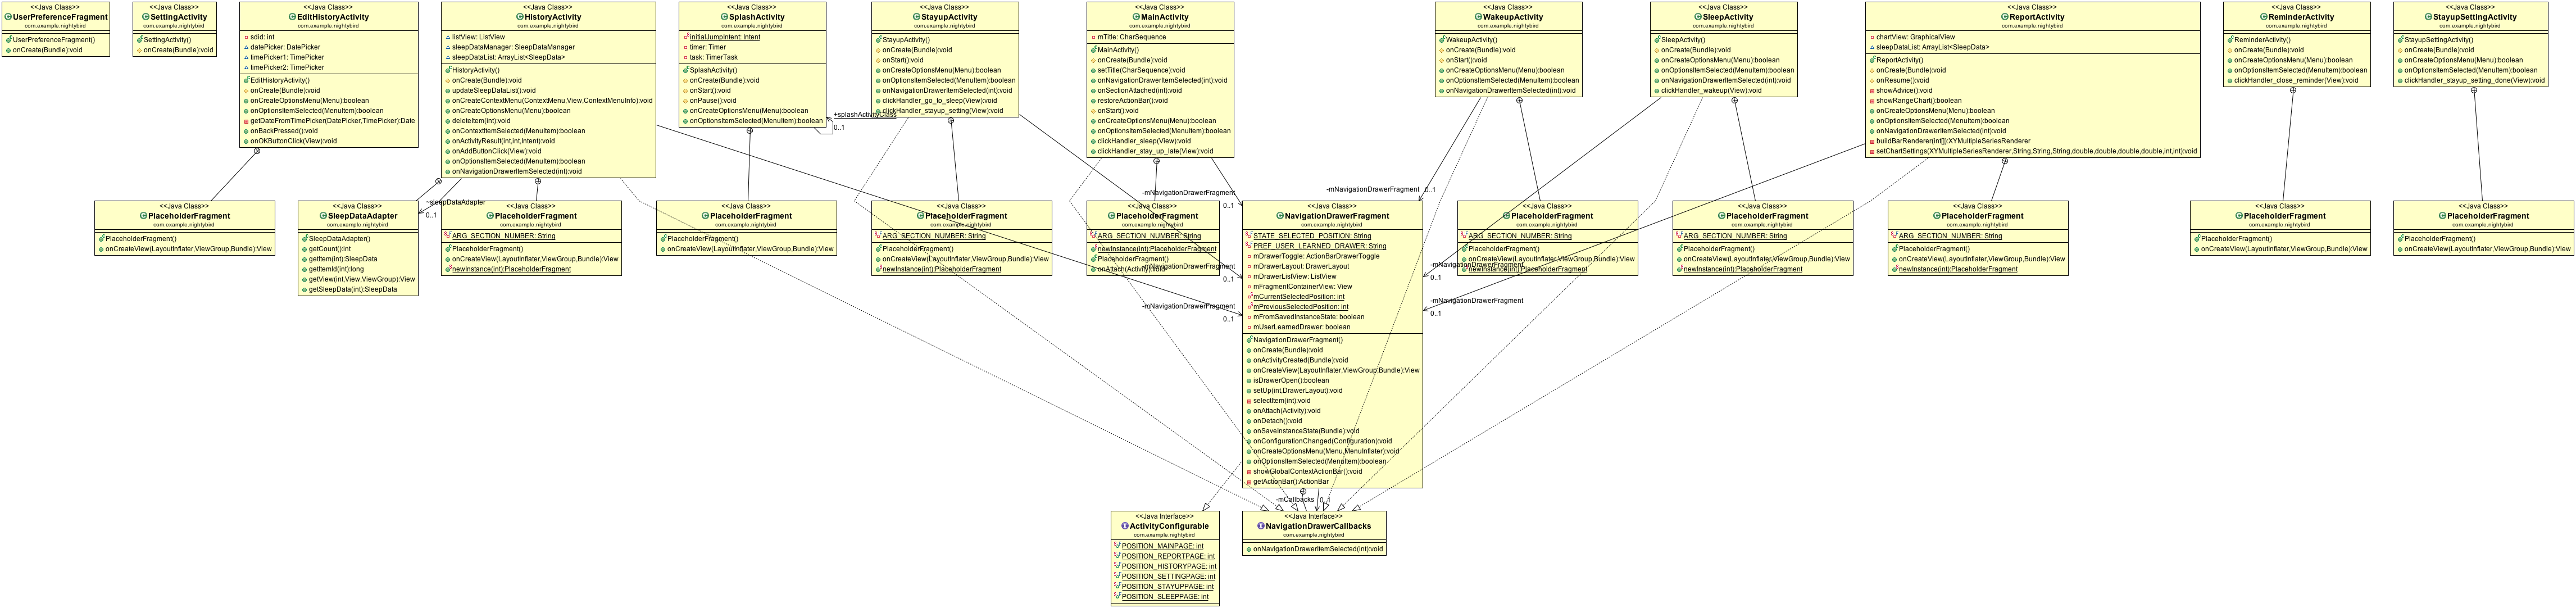
\includegraphics[width=6in,height=3in]{ClassDiagramForAcitivites}
\end{center}
\caption[Class Diagram for Acitivites]{Class Diagram for Acitivites}
\end{figure}

\begin{figure}[h]
\begin{center}
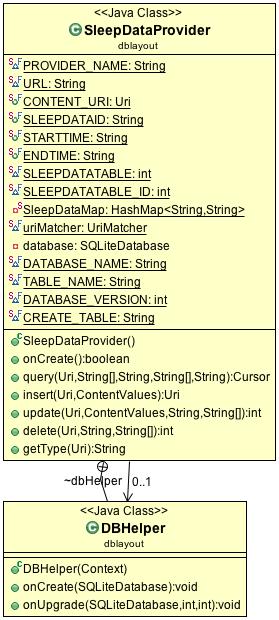
\includegraphics[width=3in]{ClassDiagramForDB}
\end{center}
\caption[Class Diagram for Database Layout]{Class Diagram for Database Layout}
\end{figure}

\begin{figure}[h]
\begin{center}
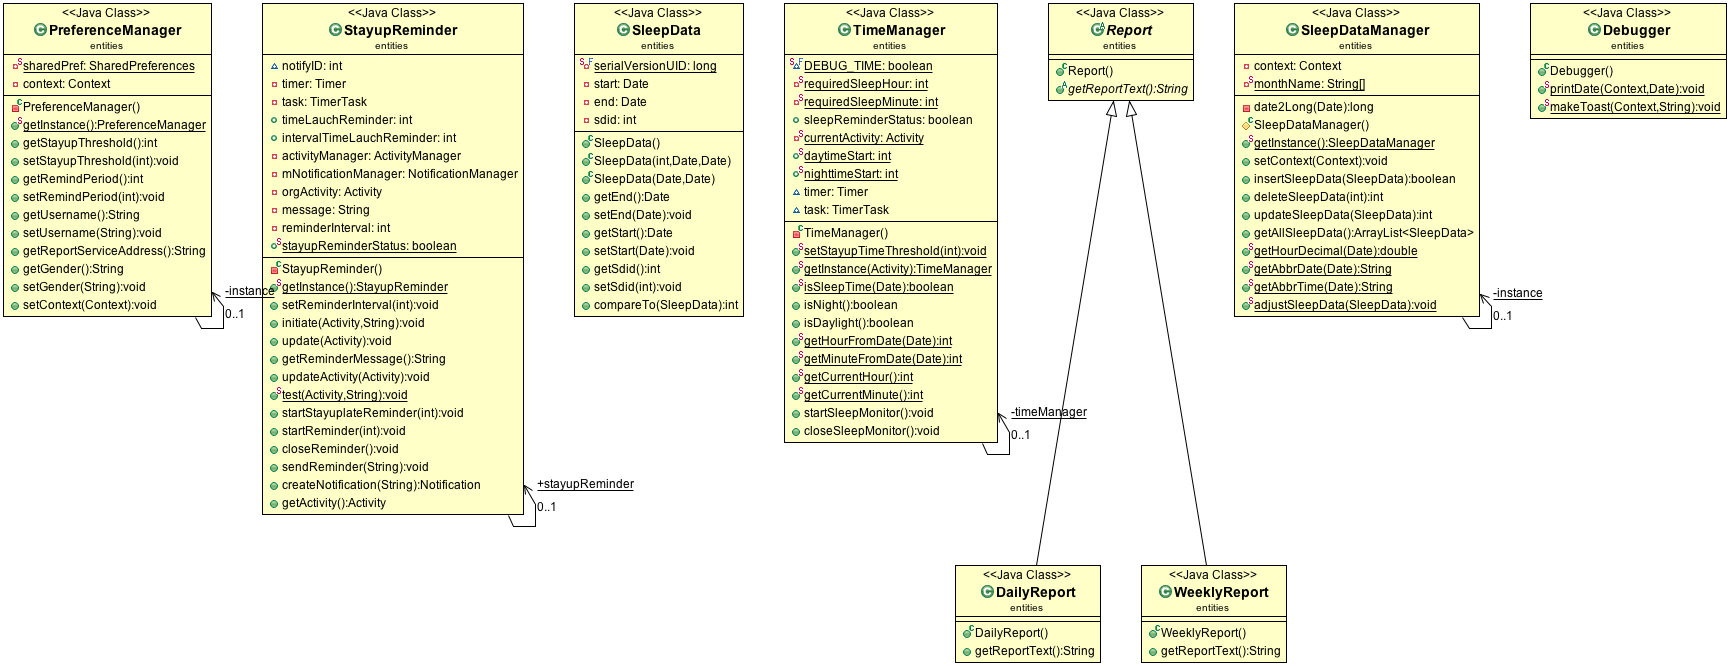
\includegraphics[width=6in,height=3in]{ClassDiagramForEntities}
\end{center}
\caption[Class Diagram for Entites]{Class Diagram for Entities}
\end{figure}

\begin{figure}[h]
\begin{center}
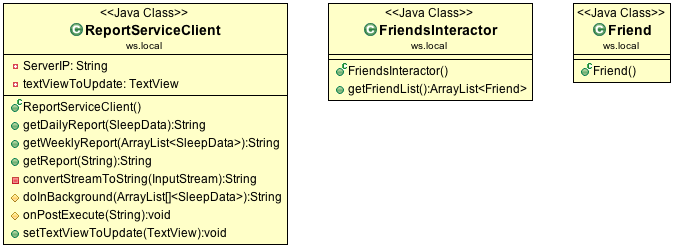
\includegraphics[width=5in,height=2in]{ClassDiagramForWebService}
\end{center}
\caption[Class Diagram for Web Service]{Class Diagram for Web Service}
\end{figure}

You can go to doc/figures for class diagrams of higher resolution.

\chapter{User Interfaces}
We have four main views: main, report, history and settings views and a navigation drawer fragment that user can use to navigate between the four views. A preference fragment is attached to setting activity and a history editor activity is triggered by the history activity. 

Here's the screen shot for our navigation drawer.
\begin{figure}[h]
\begin{center}
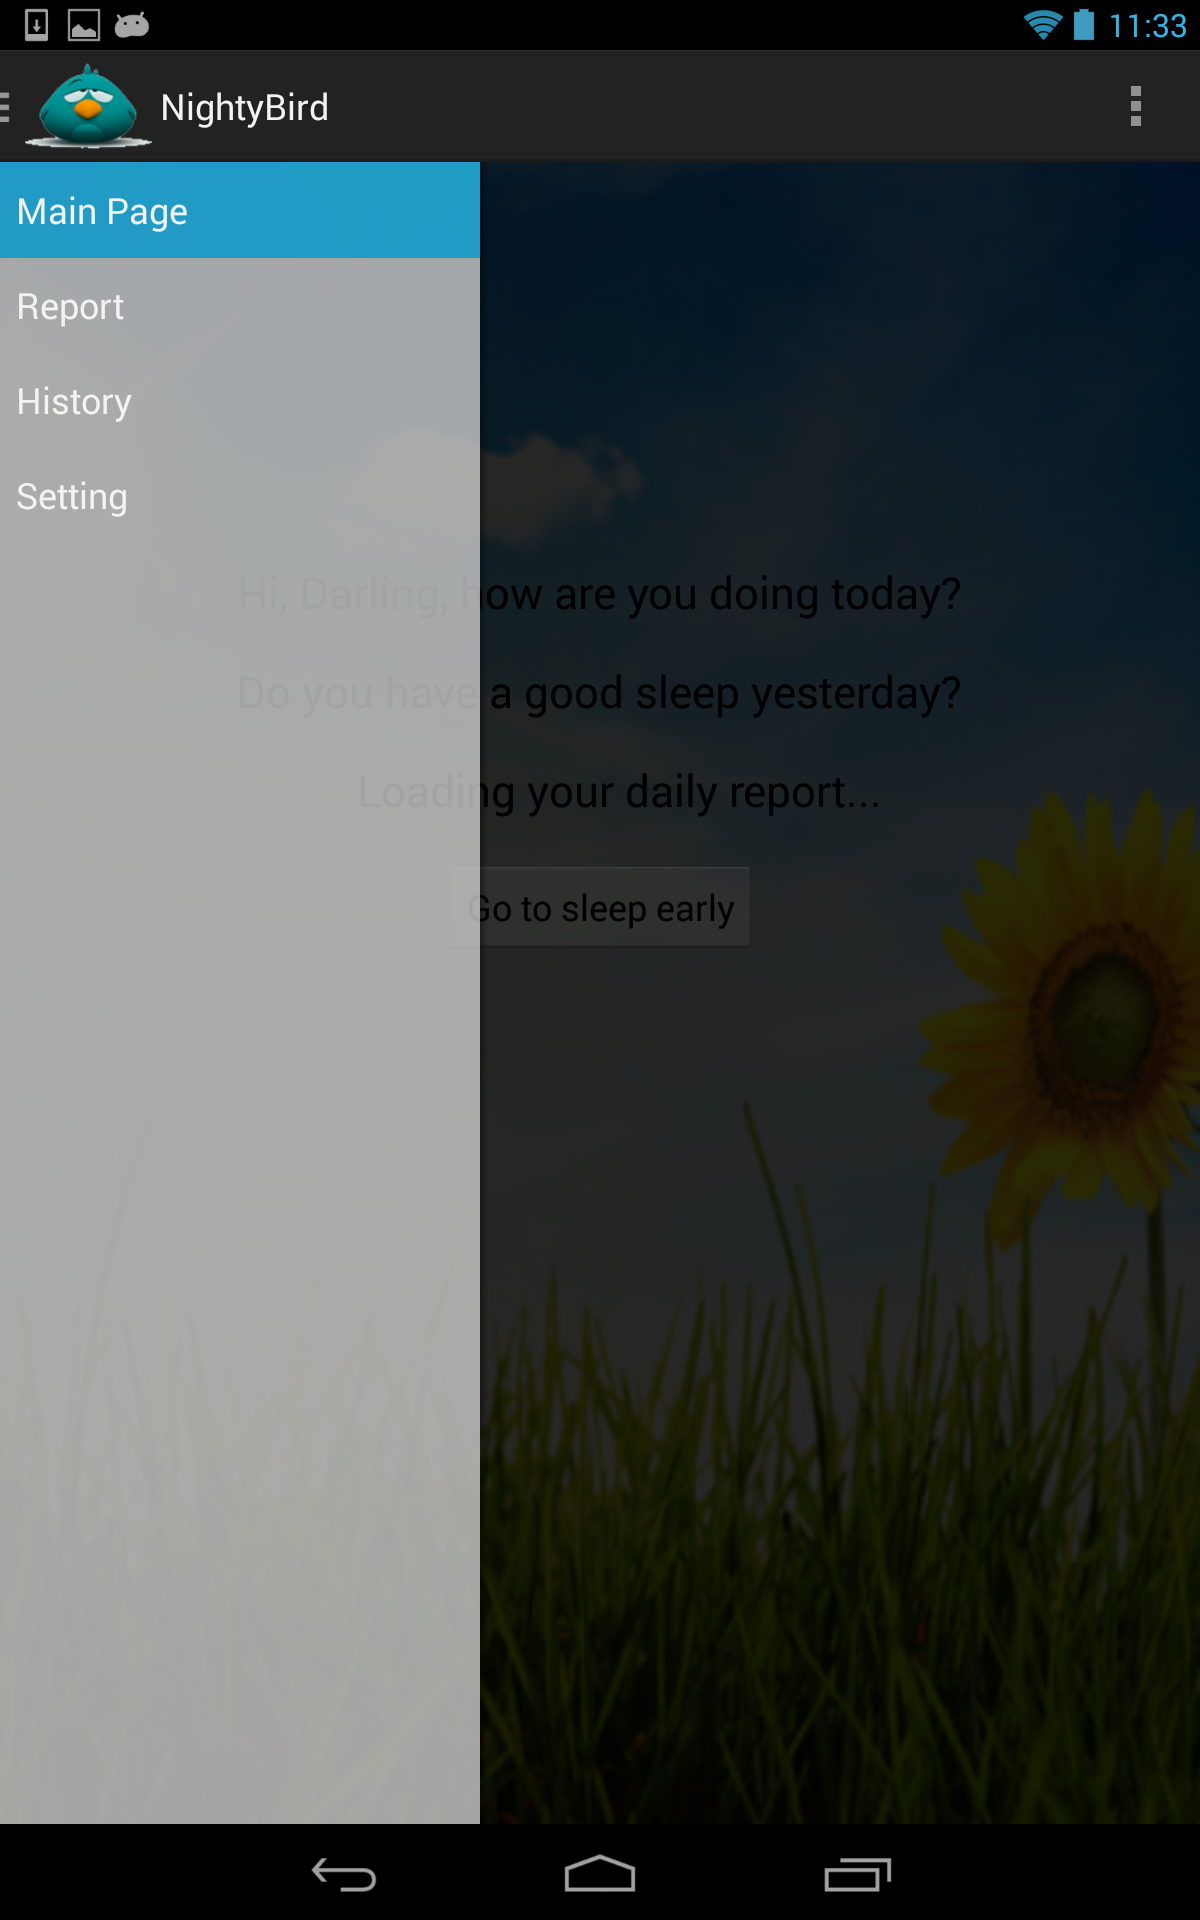
\includegraphics[width=5in]{drawer}
\end{center}
\end{figure}

\chapter{Main Page and Reminder}
Main view can present different activities based on local time on android phones. While WakeupActivity appears on the main page in daylight, StayupActivity occupies the main page after the stay-up-late threshold time at night. If users click "go to sleep" button in StayupActivity, main page shows SleepActivity. If user click "I am waken up" button, main page shows WakeupActivity. 

\begin{figure}[h]
\begin{center}
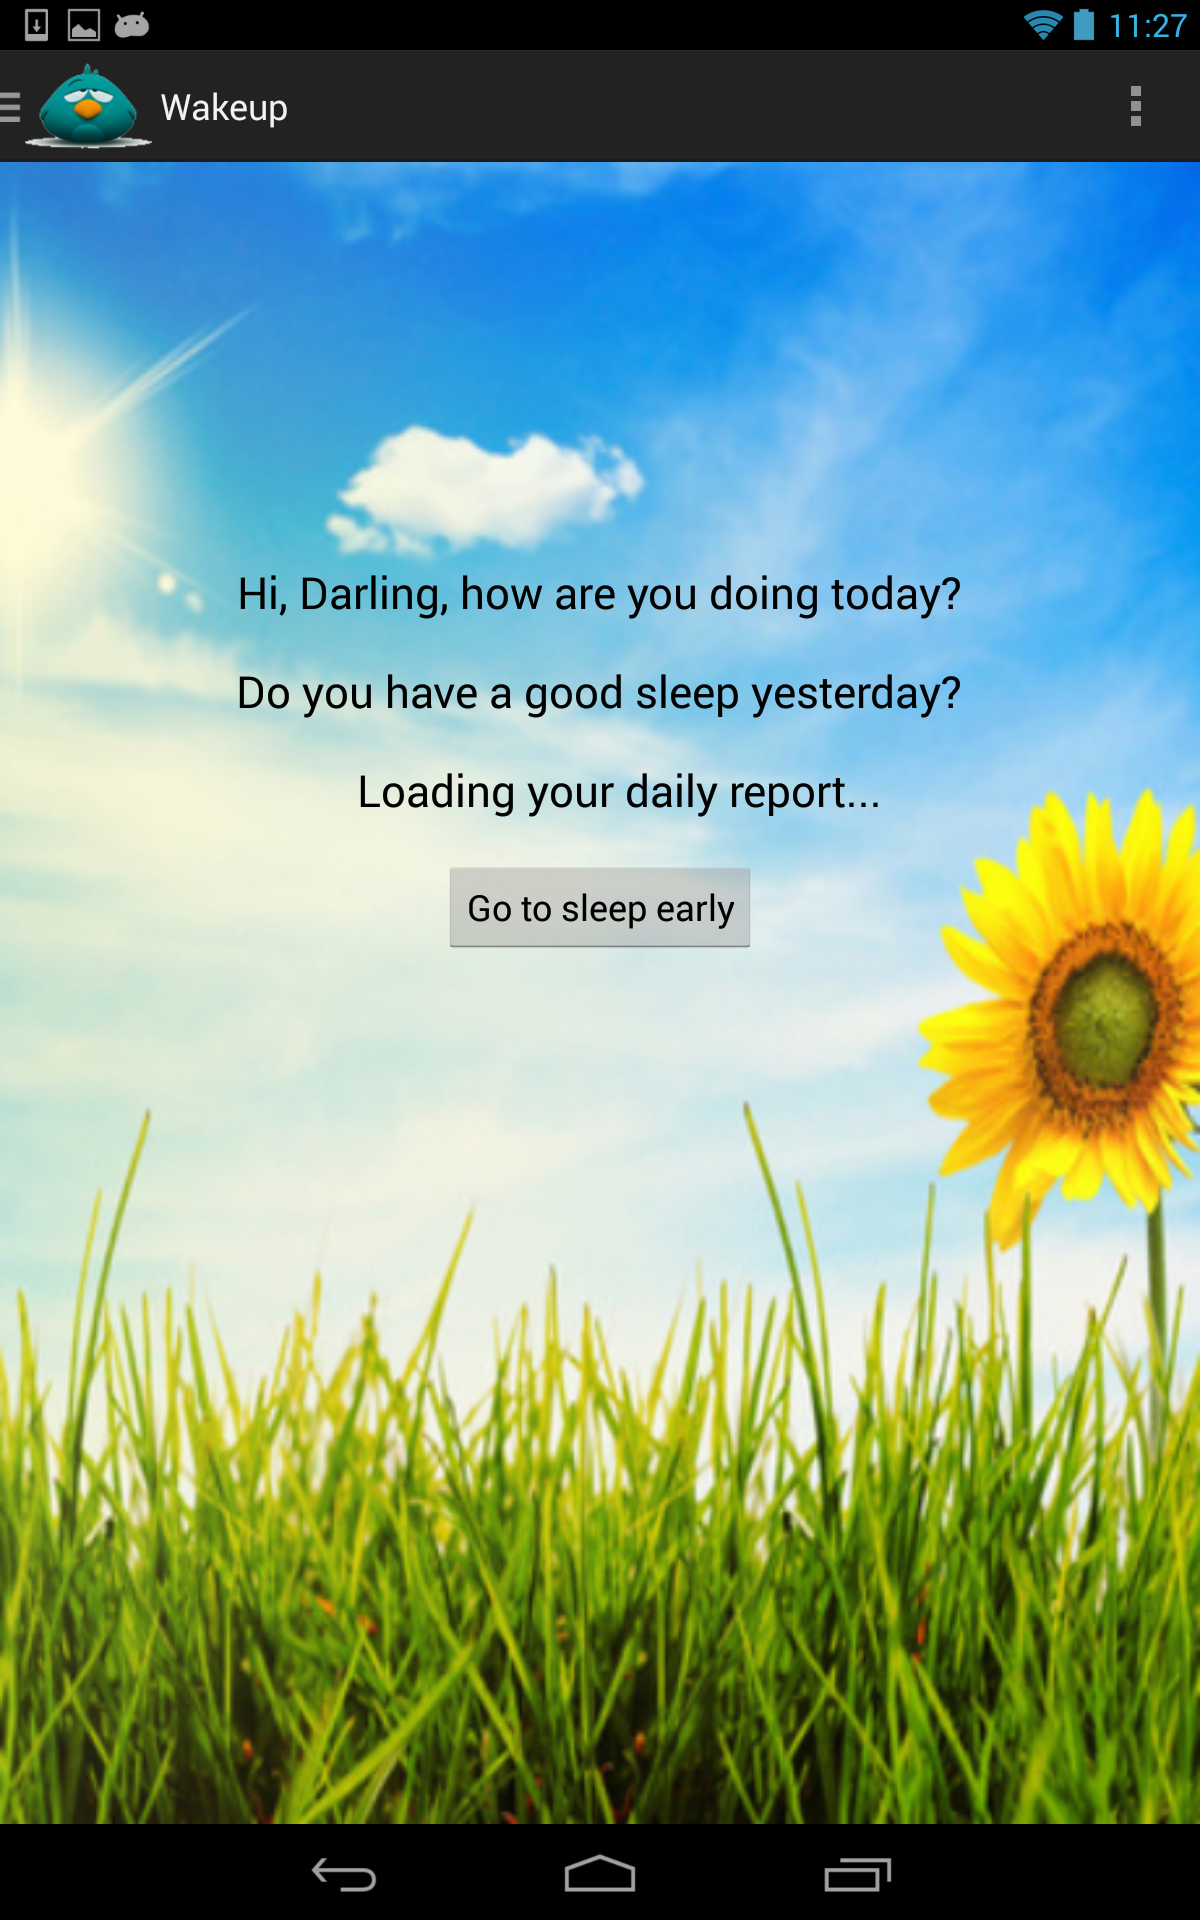
\includegraphics[width=5in]{wakeup}
\end{center}
\end{figure}

\begin{figure}[h]
\begin{center}
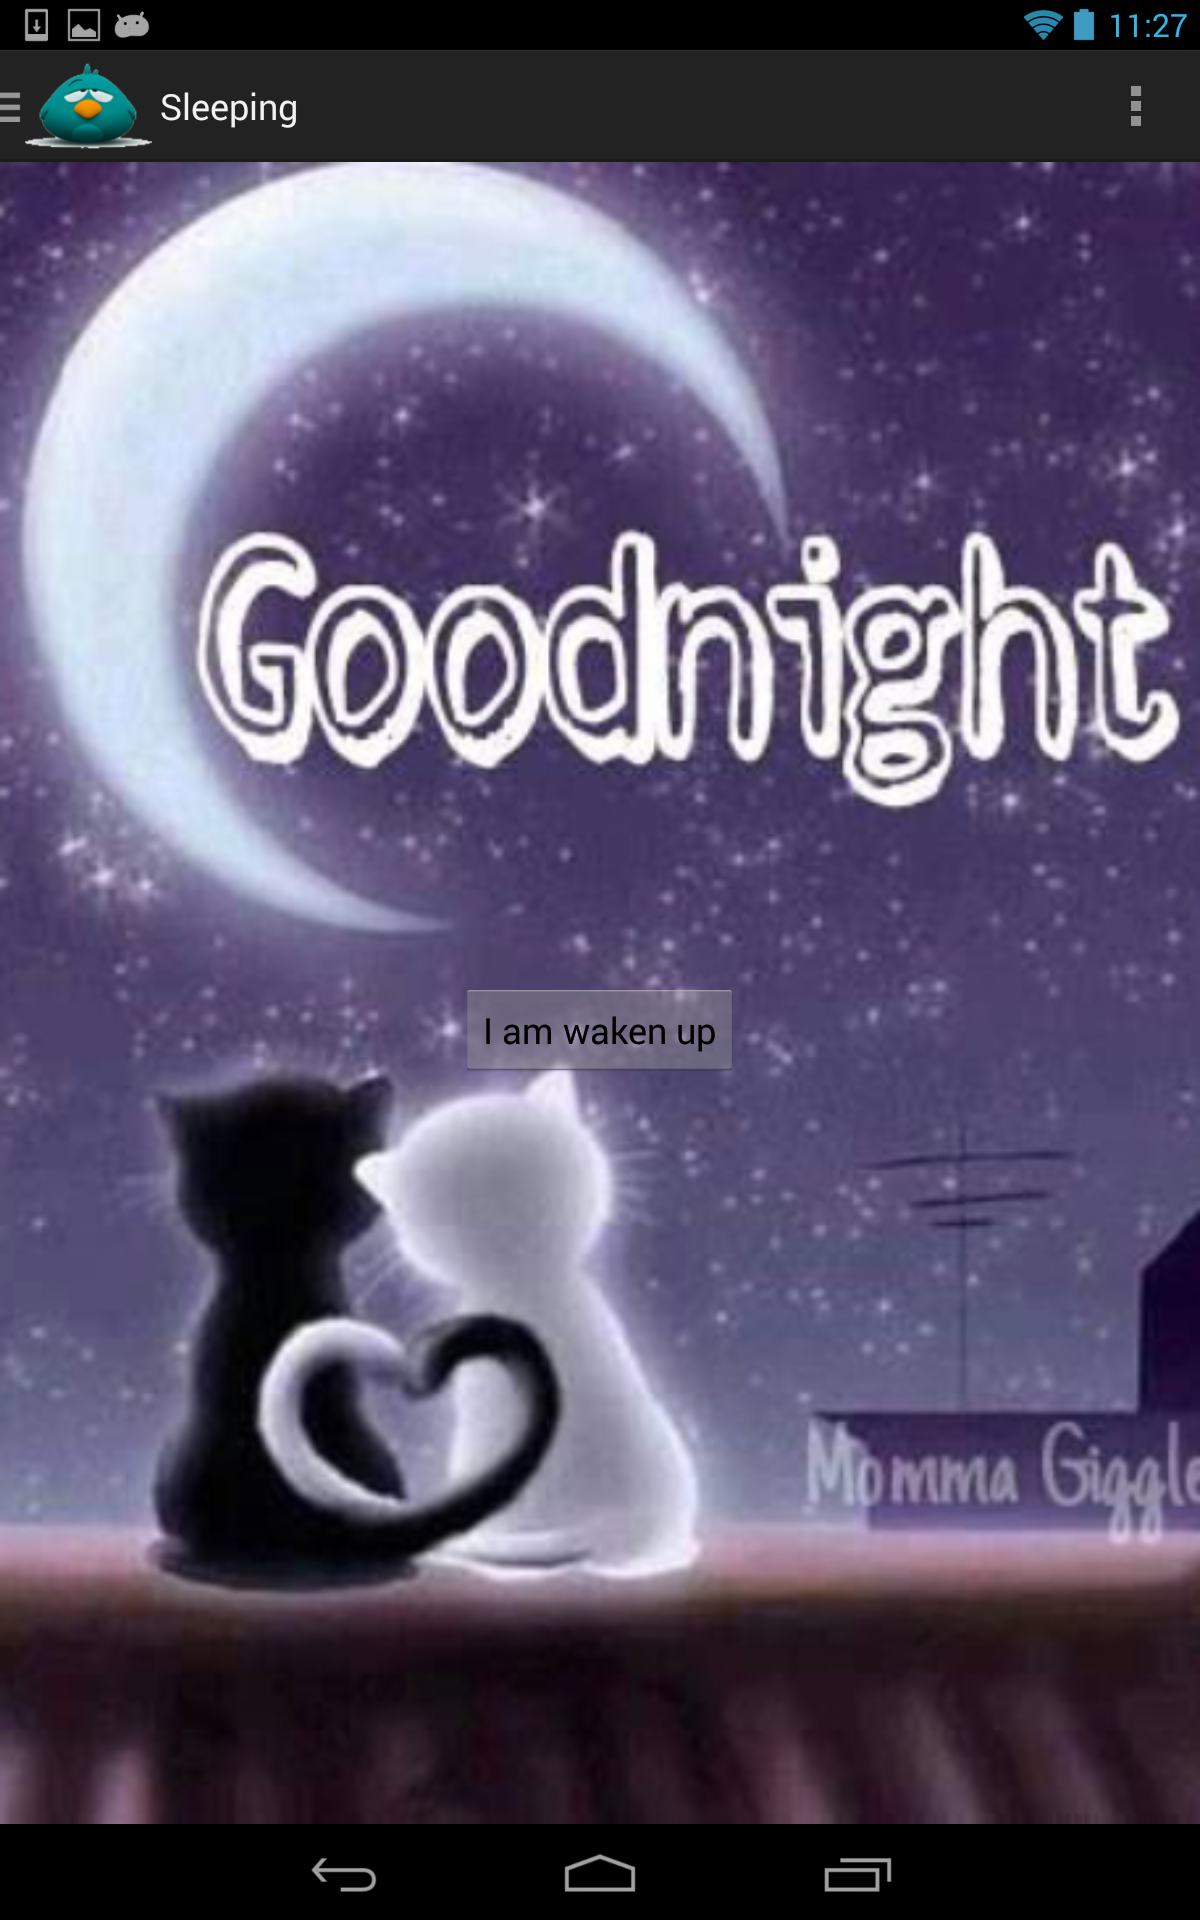
\includegraphics[width=5in]{sleep}
\end{center}
\end{figure}

\begin{figure}[h]
\begin{center}
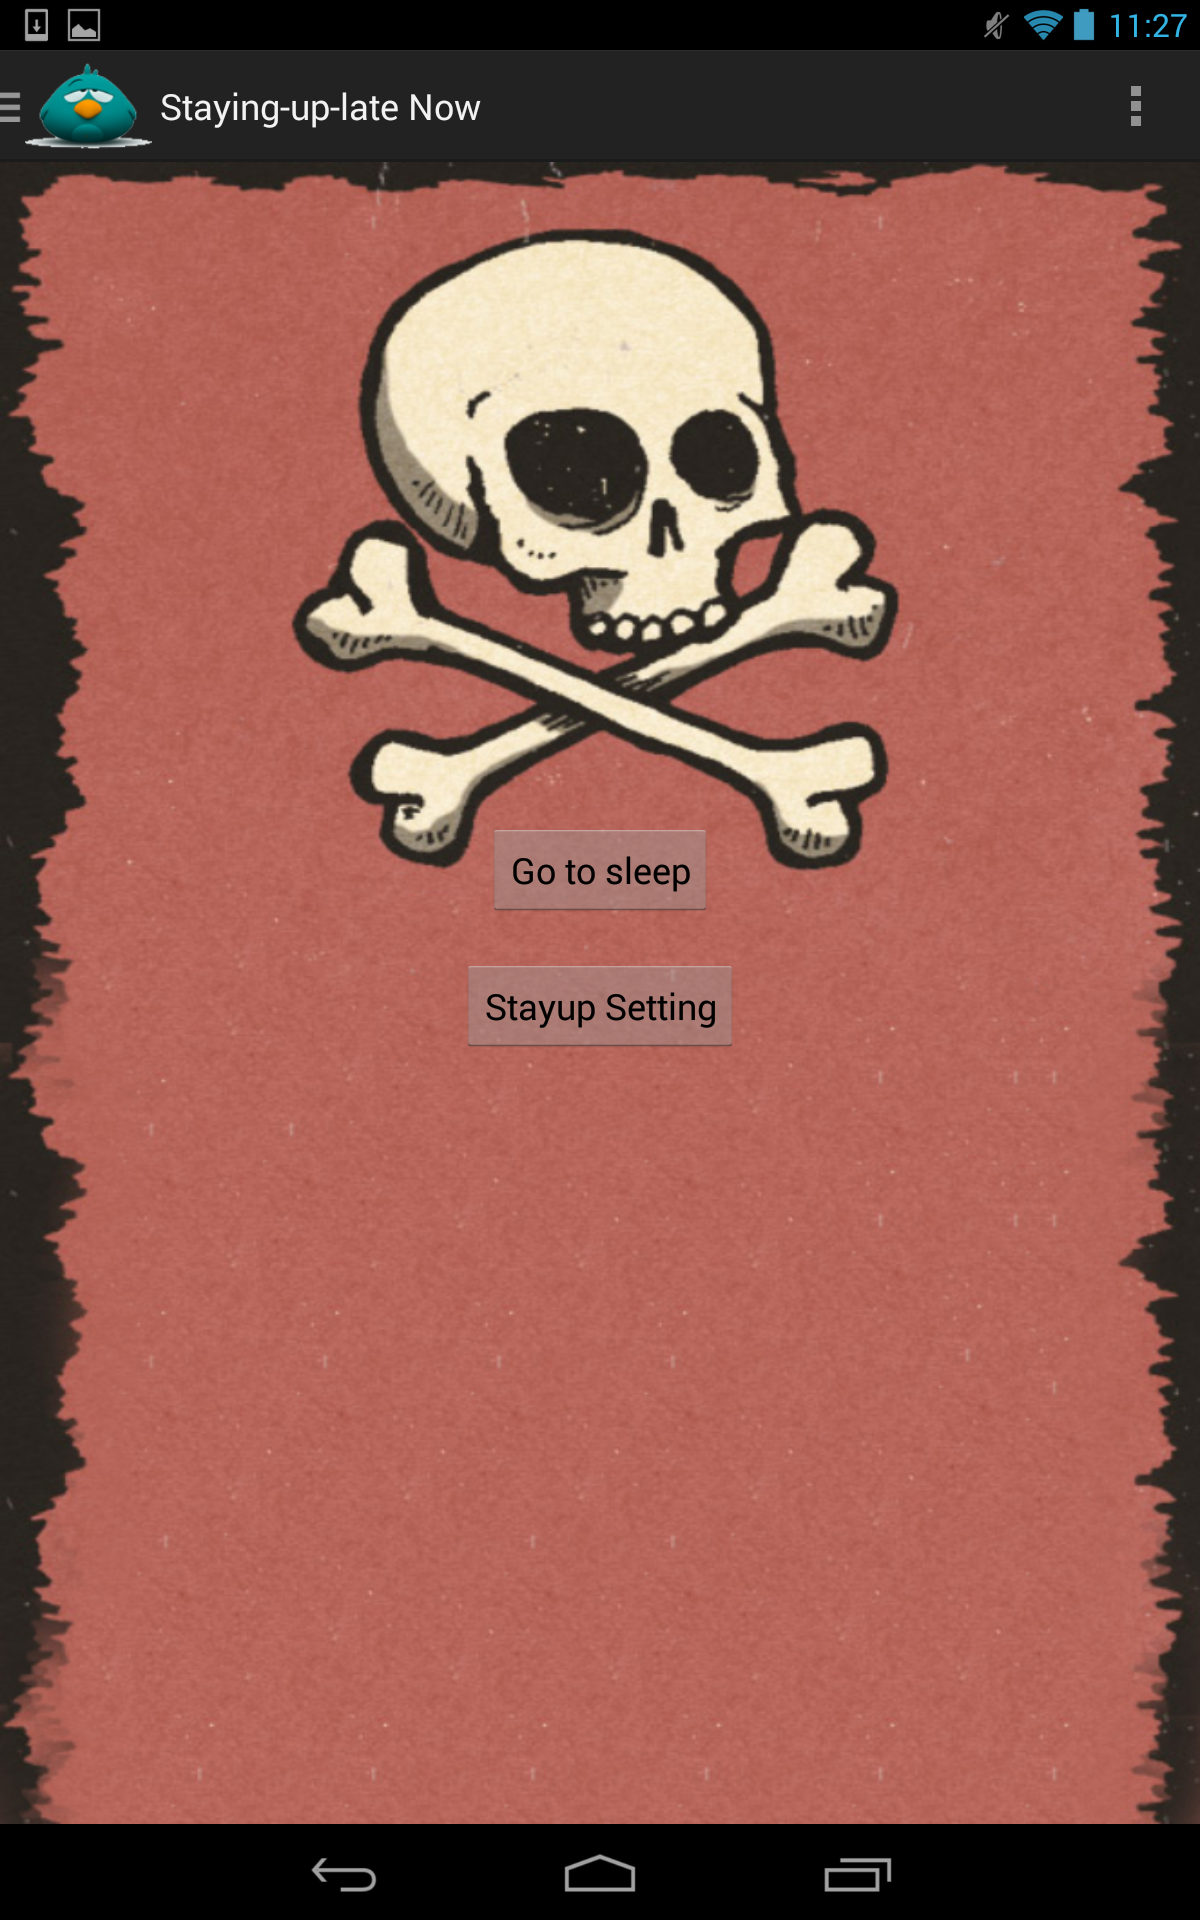
\includegraphics[width=5in]{stauplate}
\end{center}
\end{figure}

\begin{figure}[h]
\begin{center}
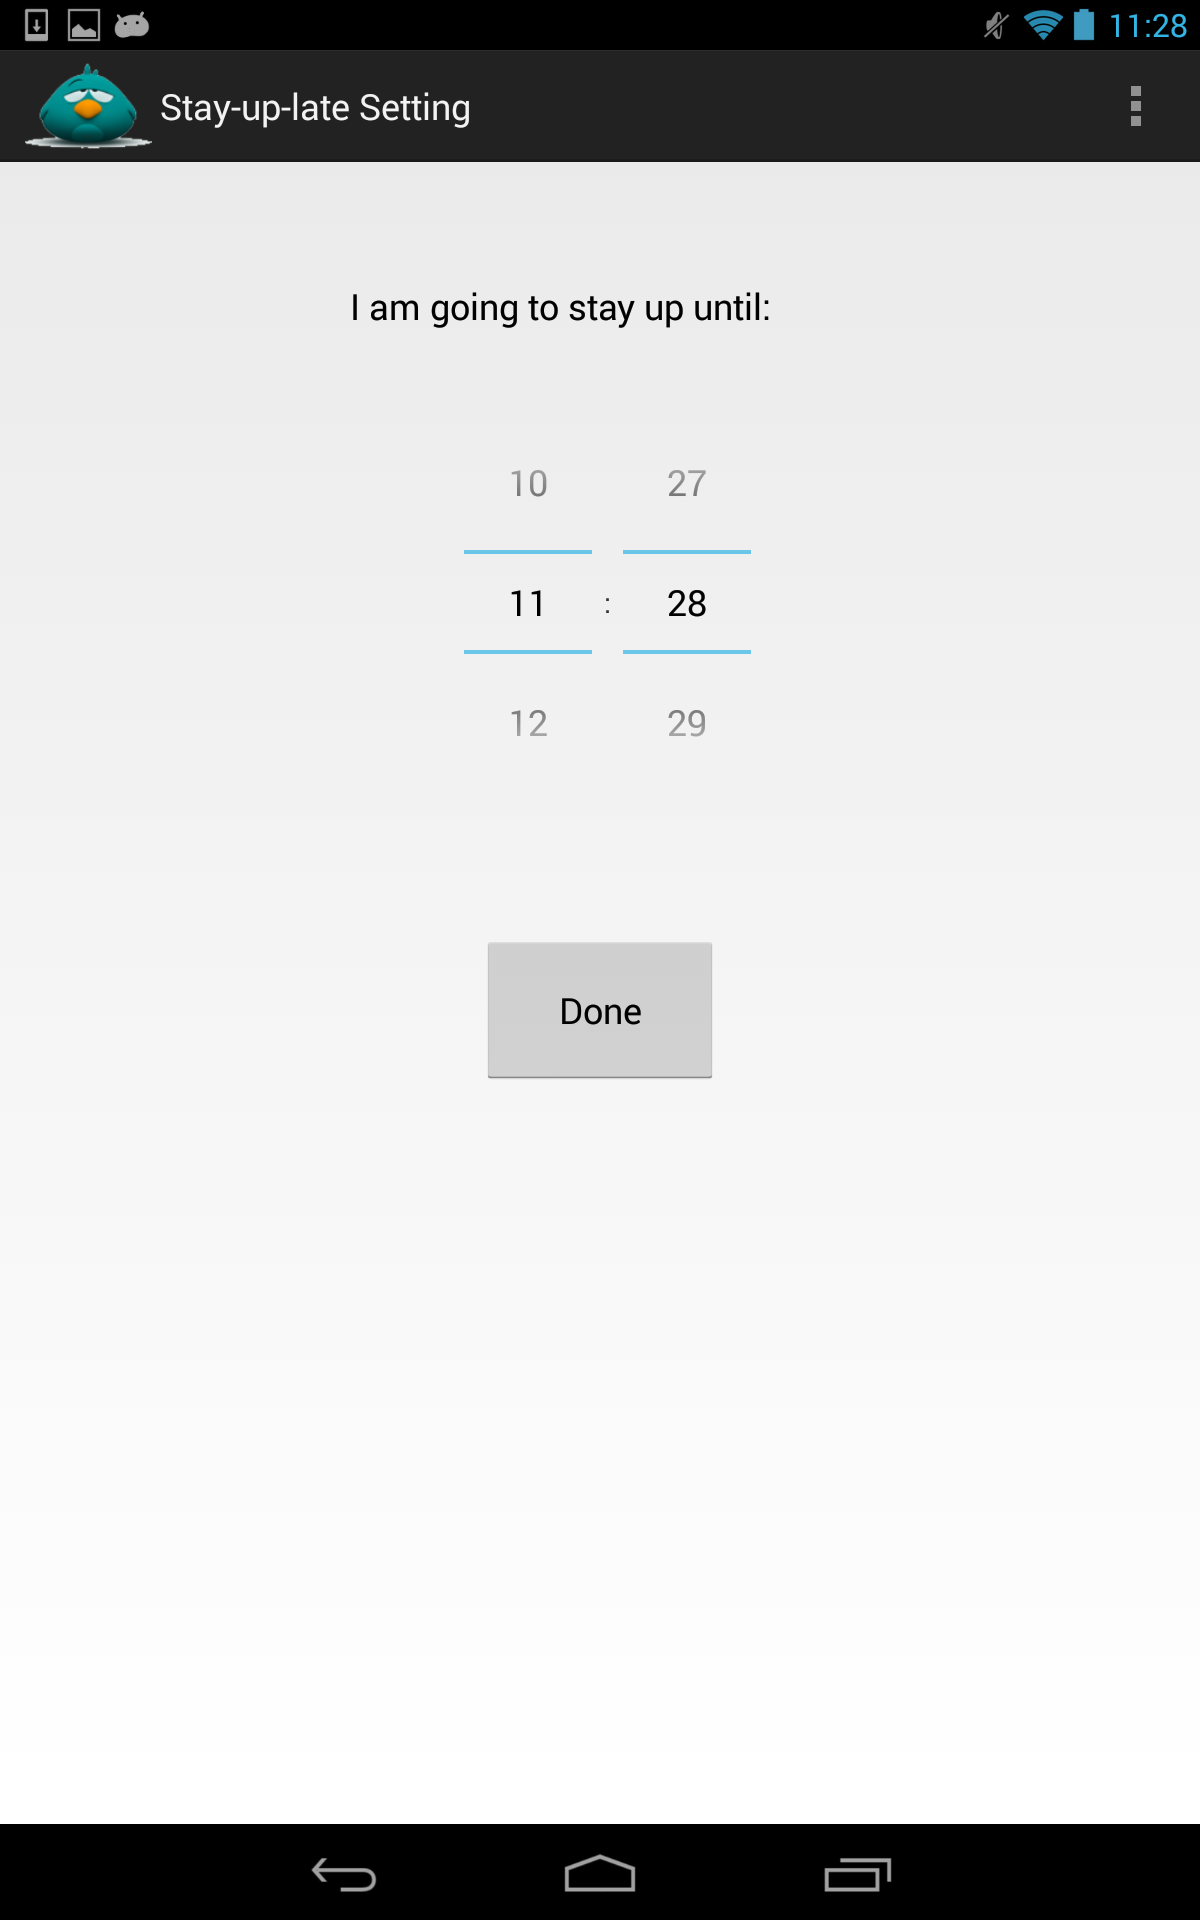
\includegraphics[width=5in]{stayuplate_setting}
\end{center}
\end{figure}

\section{TimeManager}
TimeManager realized singleton pattern. It includes a series methods to analyze current time and some a methods to start Sleep Monitor. Sleep Monitor is running as a thread and give notification when it is time to sleep.

\section{StayupReminder}
StayupReminder is also of singleton pattern. It includes methods to give notification on the phone, which we called reminder. Reminder could include sound, vibration and text. Users can set StayupReminder in StayupActivity, indicating when to terminate stay up late. Also, StayupReminder could be reused by TimeManager to implement Sleep Monitor.

\begin{figure}[h]
\begin{center}
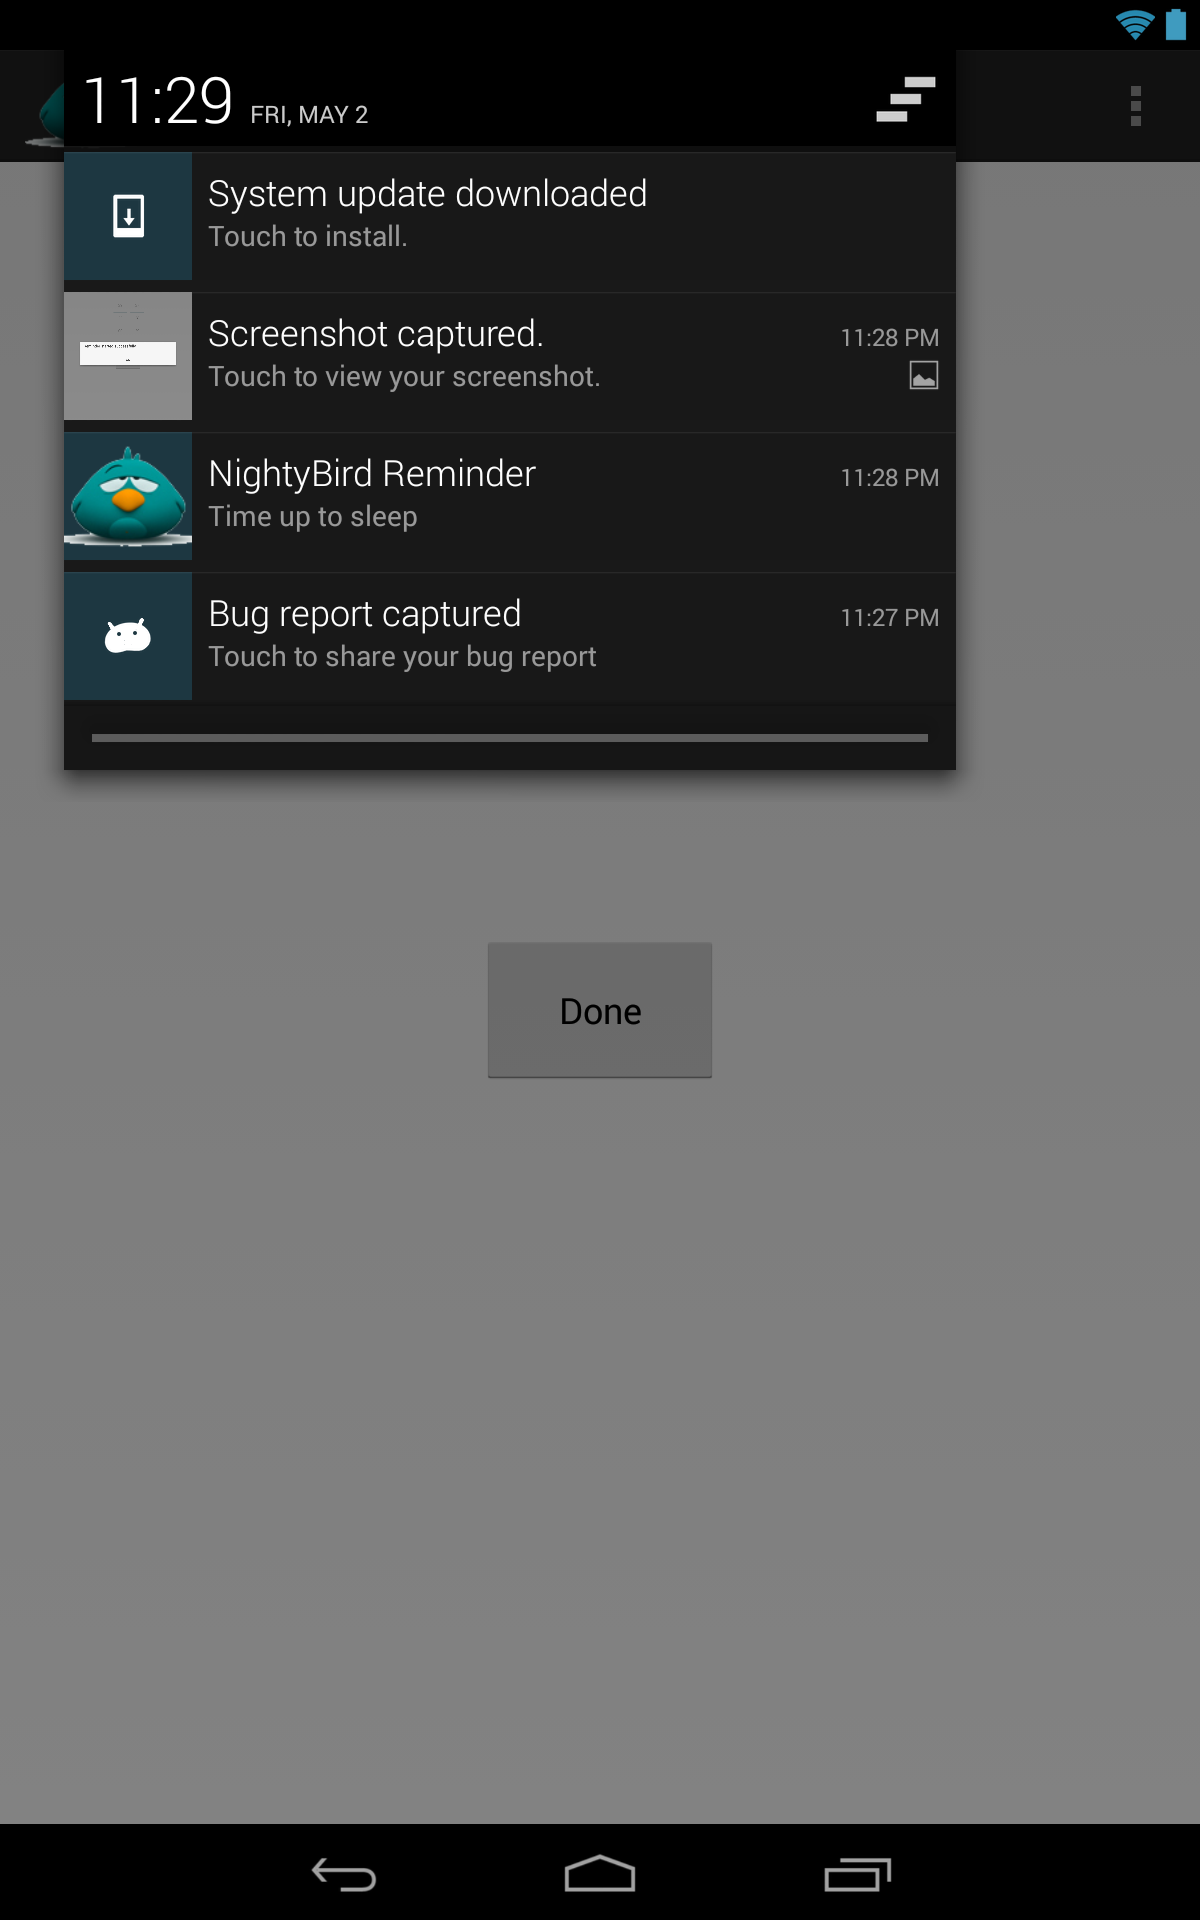
\includegraphics[width=5in]{reminder}
\end{center}
\end{figure}

\begin{figure}[h]
\begin{center}
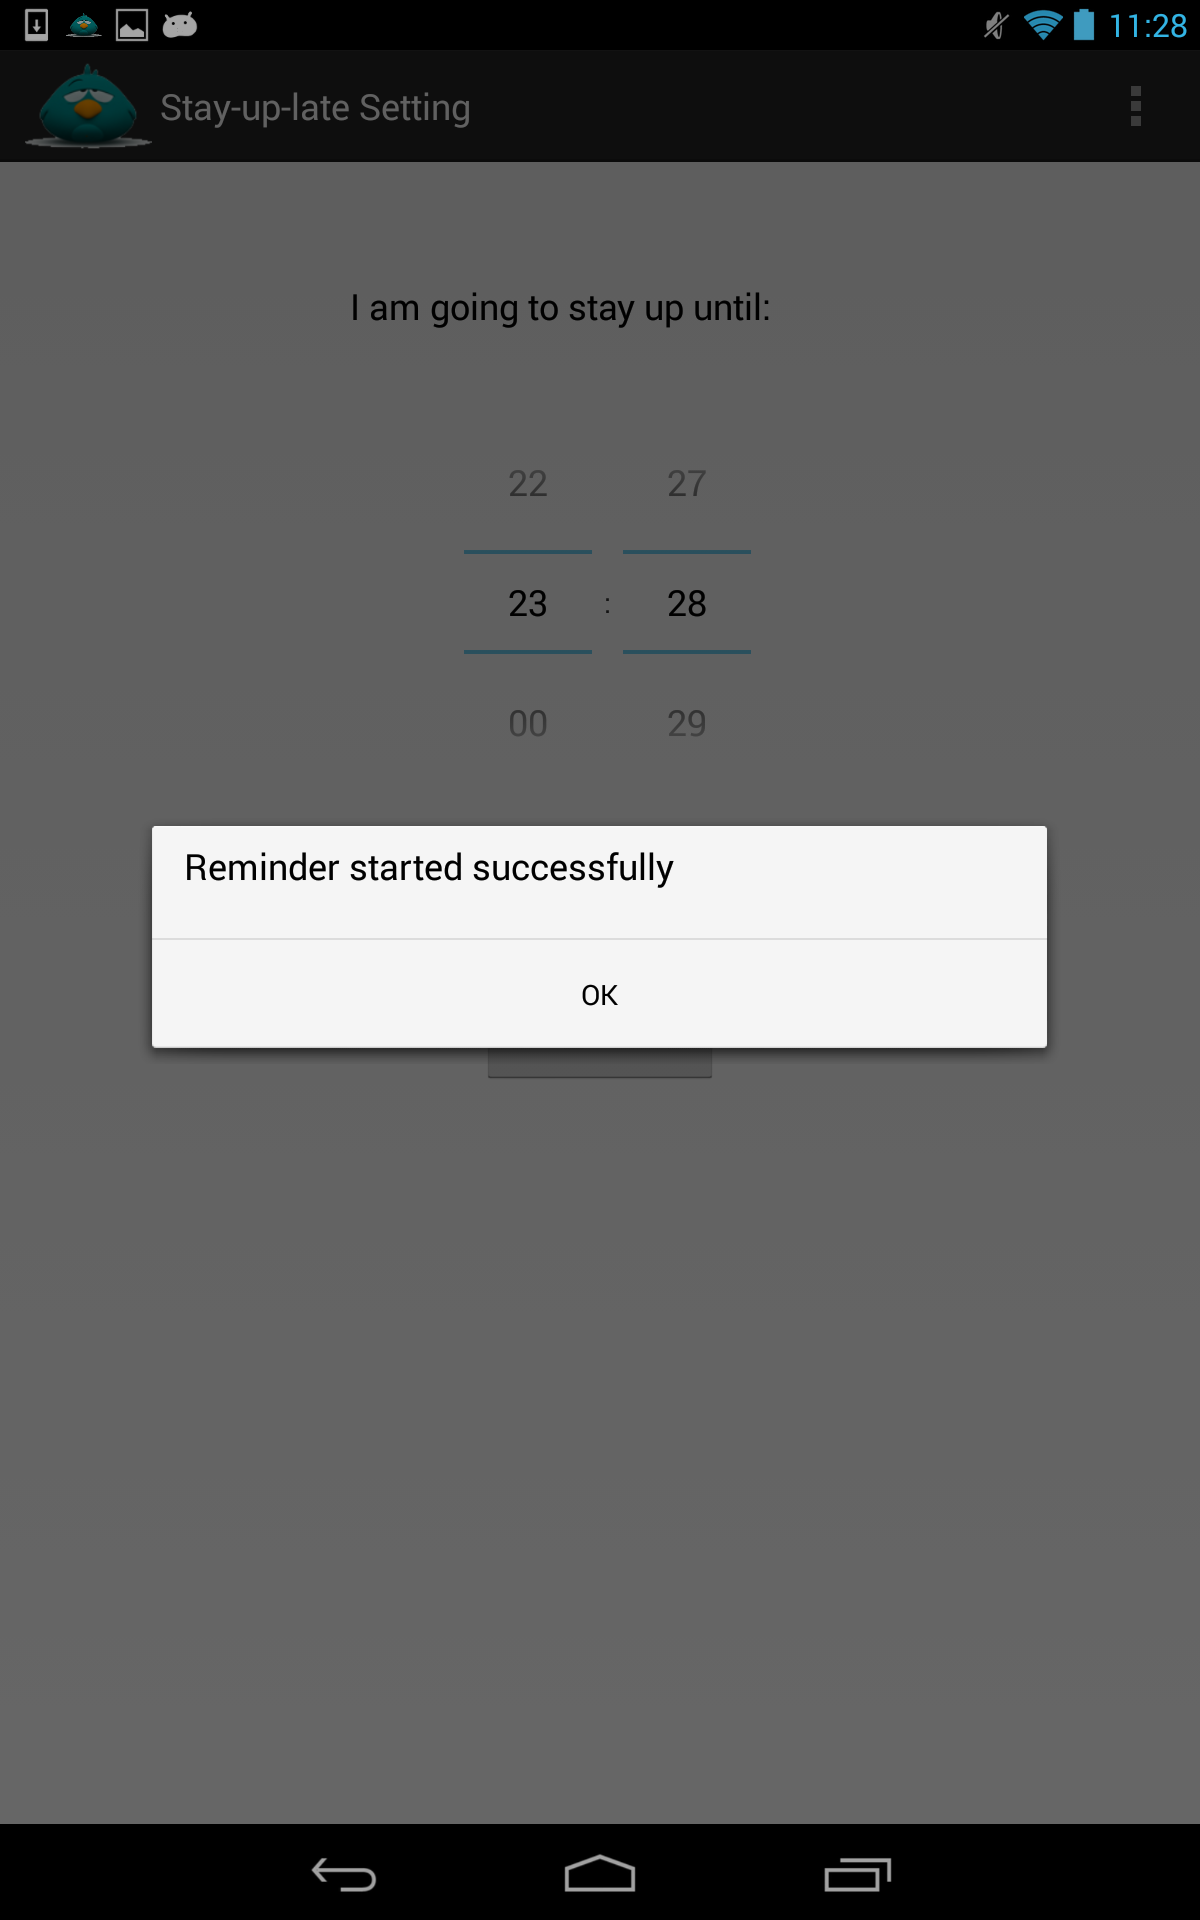
\includegraphics[width=5in]{reminder_started}
\end{center}
\end{figure}

\begin{figure}[h]
\begin{center}
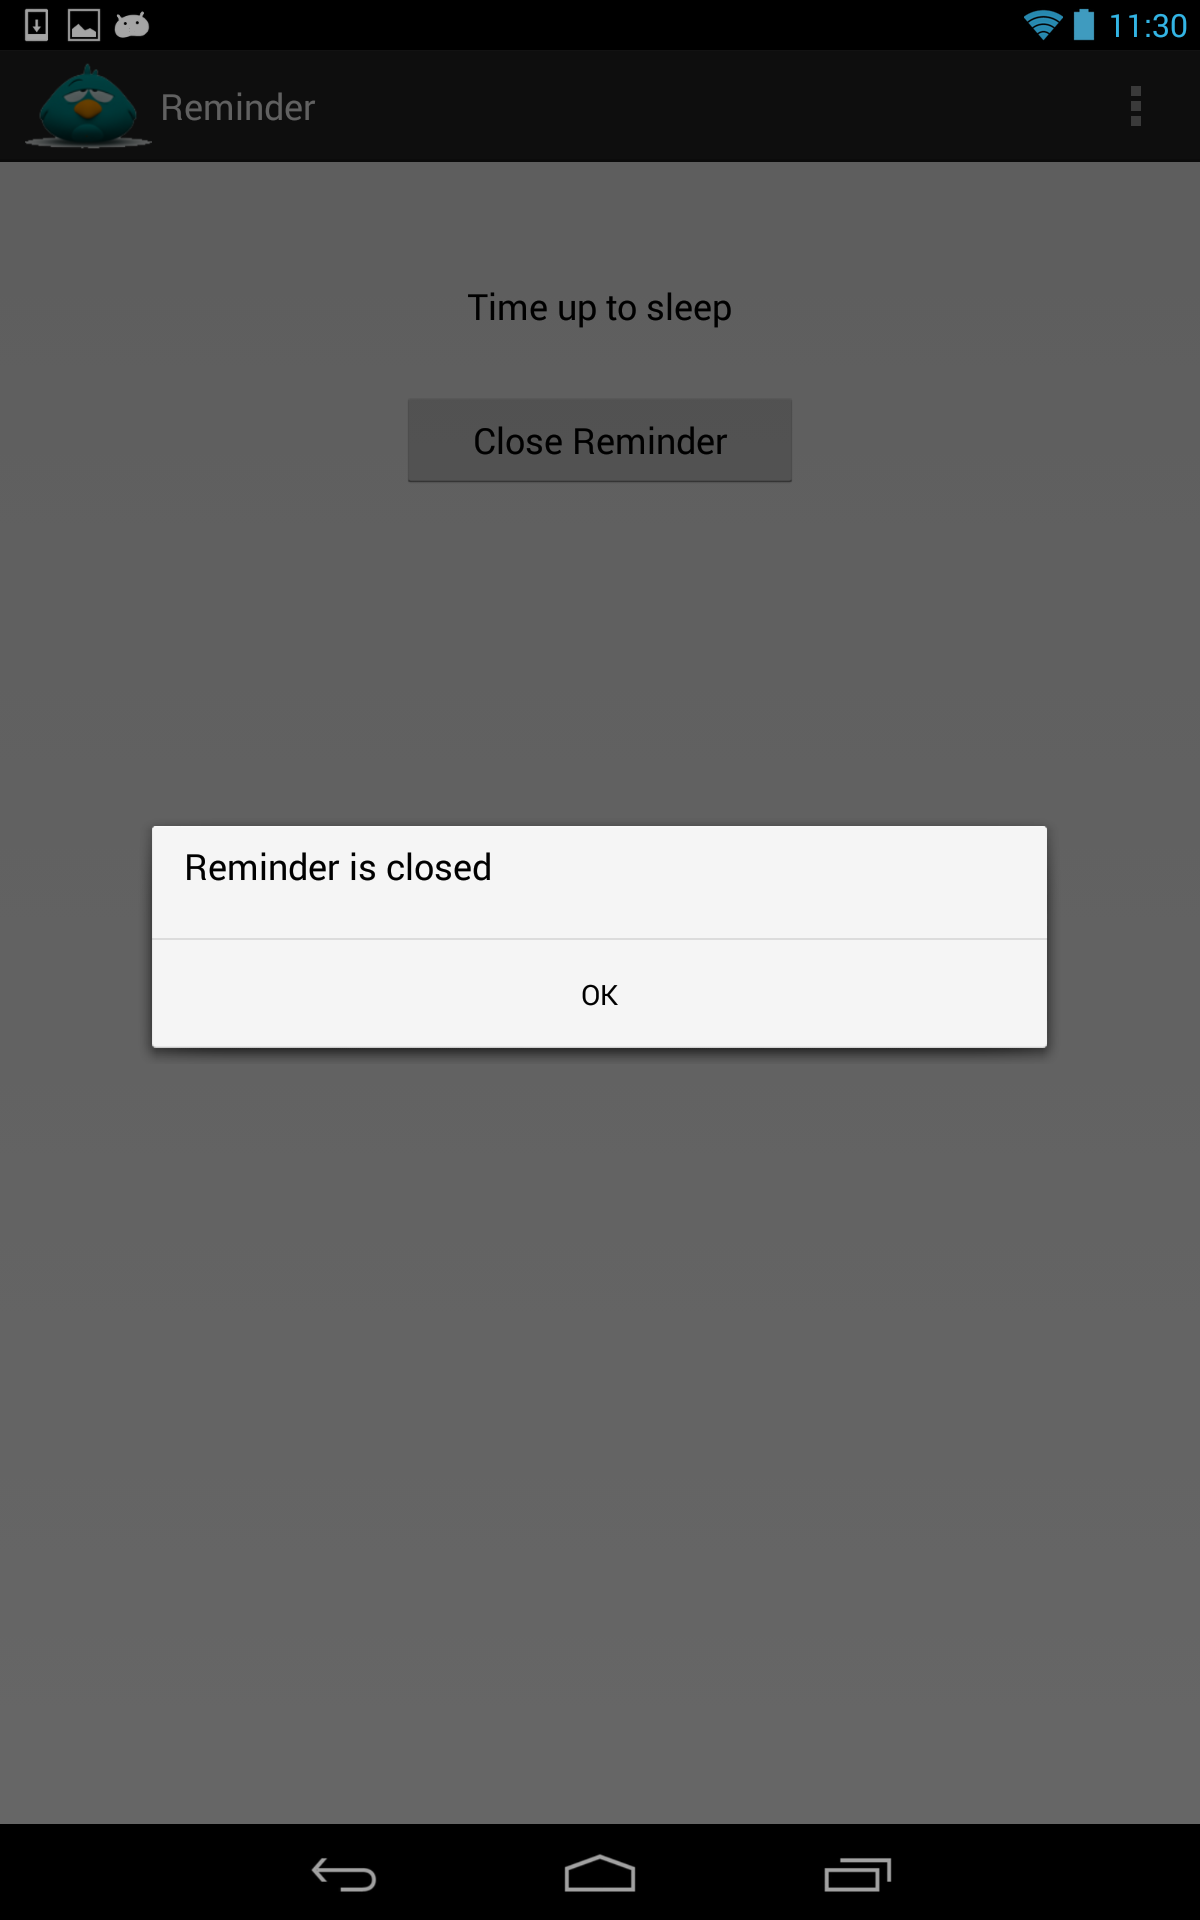
\includegraphics[width=5in]{reminder_closed}
\end{center}
\end{figure}

\chapter{Report}
On the report page, the NightyBird application presents user a weekly report as long as the user has data of at least 7 days. The report contains a range chart and a report paragraph.

\begin{figure}[h]
\begin{center}
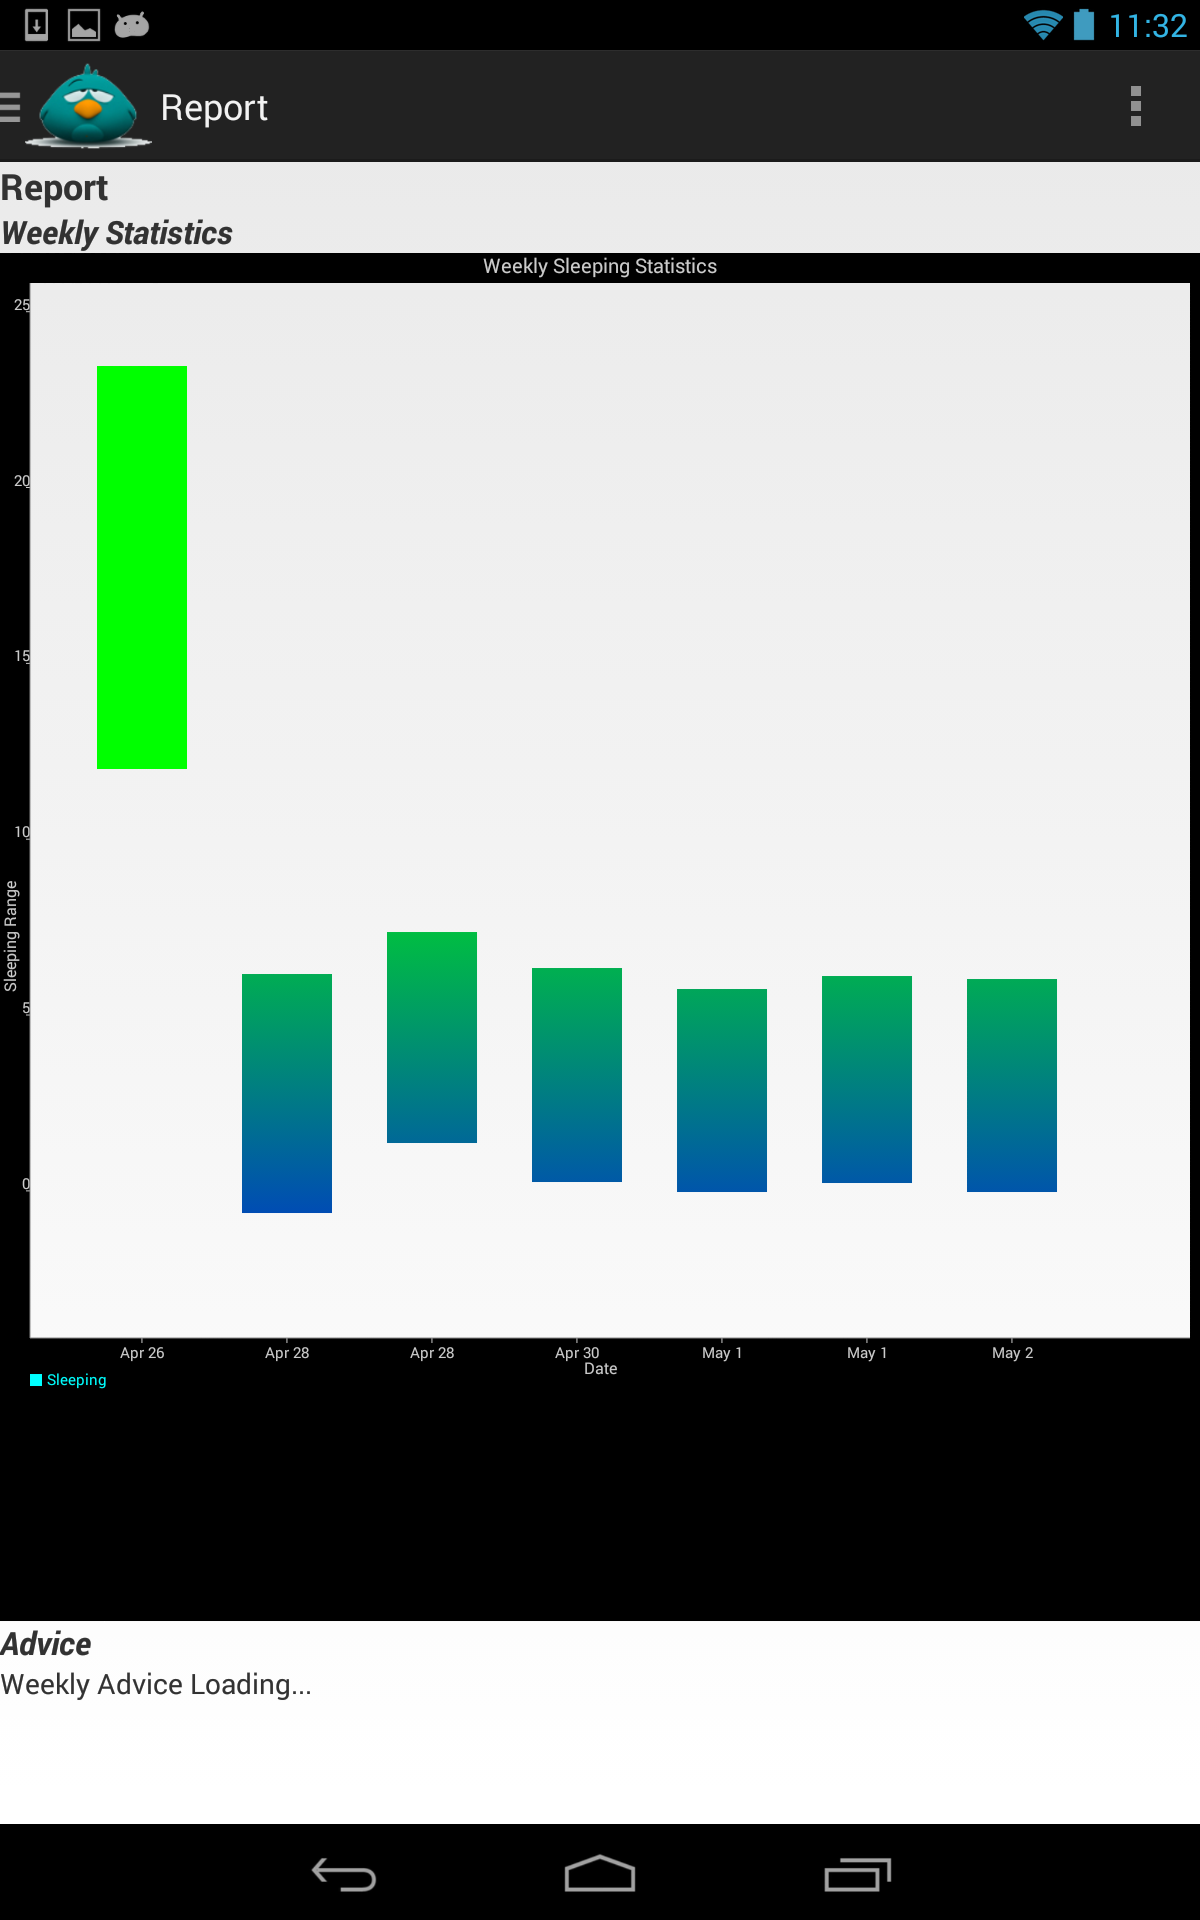
\includegraphics[width=5in]{report}
\end{center}
\end{figure}

\section{Weekly Range Chart}
The range chart includes 7 sleeping range of the past week. We use an external library AChartEngine to draw the chart for us. The chart will be drawn on creation or resume of the report activity.

\section{Report Web Service}
There's a text view below the range chart. We use this text view to present our advices for this user. The text of this text view is dynamically loaded via report web service. Every time the report activity is created or resumed , the report service client (ReportServiceClient) will be invoked to fetch advice text from server. 

\section{The Client}
The client is implemented by ReportServiceClient class which extends android.os.AsyncTask. Therefore, the client will execute its task in the background task other than in the activity thread.

To use this client, we pass an TextView object into it and starting executing asynchronously. In it task, it send a http request to the the server and server will response with a JSON string.  The http request will contain the user's sleep data, either daily data or weekly data. The JSON string will parsed into a JSON object, a field called "report" will be fetched and the preset text view will be set the text to be the content of the report.

The server ip can be configured by users in the setting activity.

In case of any failure like network failure, the text view will display the problem and there will be a dialogue telling user about it.

\section{The Server}
A Dynamic Web Project is built to implement the server.  The server provides two APIs: daily and weekly. The format could be listed as below:

daily  API:\\
\begin{verbatim}
domain:[Port Num]/NightyBird_Server/daily?start=[Date]&end=[Date]
\end{verbatim}

weekly API:\\
\begin{verbatim}
domain:[Port Num]/NightyBird_Server/weekly?
start1=[Date]&end1=[Date]&start2=[Date]&end2=[Date]
&start3=[Date]&end3=[Date]&start4=[Date]&end4=[Date]
&start5=[Date]&end5=[Date]&start6=[Date]&end6=[Date]
&start7=[Date]&end7=[Date]
\end{verbatim}

As for daily API, server analyzes whether the starting sleep time is late and how long users sleep in the specific day. As for weekly API, server analyzes average sleep time in the week. Response from server is in form of JSON, which enable to server to extend information in response. The response by now is in the form:
\begin{verbatim}
{"report":"[report text]", "error":"[error text]"}
\end{verbatim}


\chapter{Database and Sleep Data History}

\section{Schema}
We a content provide to maintain user's sleep data. We have structured sleep data class called SleepData that contains a start time, an end time and an id as well. This id will be filled by the inner database and it is the primary key of the sleep data table.

We define our database table as following:
\begin{verbatim}
    CREATE TABLE SleepDataTable
    (SDID INTEGER PRIMARY KEY AUTOINCREMENT, 
     StartTime LONG NOT NULL,
     EndTime LONG NOT NULL)
\end{verbatim}
The id is automatically created by the database and we fill the start time and end time by unix time. The reason we use unix time is because its a uniform time and we will not have any ambiguity across platforms and people. It is also convenient for us to compare them.

In addition to that, we also have a singleton class called SleepManager which exposes interfaces to insertion, update or deletion of the database. Besides, some utilities like converting Date class to date string are also provided.

\section{History List}
In the history activity, we use a list view to present user's sleep data. It also provides interfaces for users to add, edit or delete them.

\begin{figure}[h]
\begin{center}
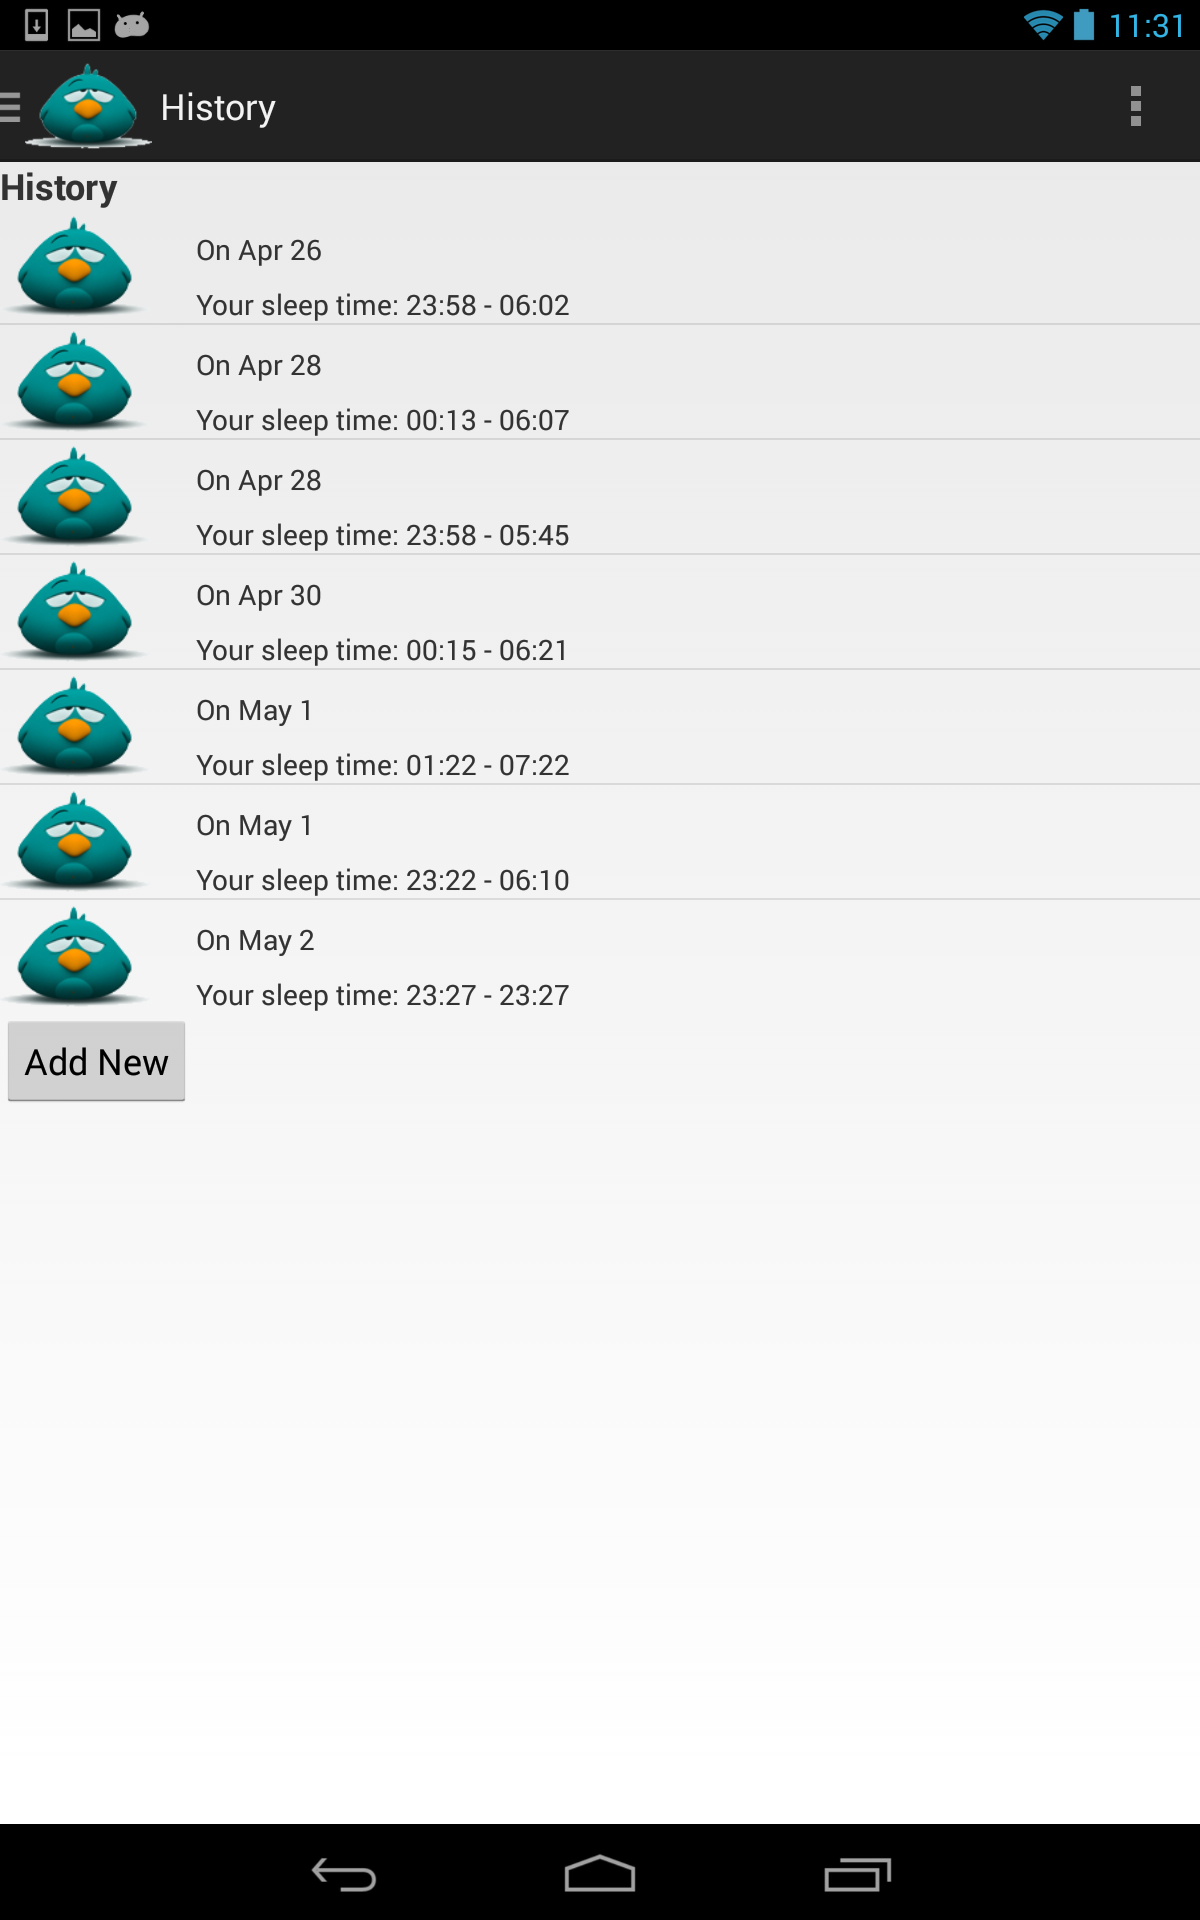
\includegraphics[width=5in]{history}
\end{center}
\end{figure}


The list view uses an adapter to get the sleep data item from database, i.e. our SleepDataManager.

Users can click Add New button to add an item to the list or he can long-click any item of the list, then a dialogue will be pop up to prompt users to chose edit, delete or cancel. 

\begin{figure}[h]
\begin{center}
\includegraphics[width=5in]{edithistory_dialogue}
\end{center}
\end{figure}


When users chose to add or edit an item, a history editor activity will be started where users call edit his sleep data. After the operation is done, users can click OK button that will return to history activity with a result containing the sleep data. The history activity will invoke the SleepDataManager to update the sleep data table accordingly. 

The history editor contains one date picker and two time picker. It prompts users to input his sleep time and wake up time for some date. When data is loaded to our SleepDataManger, if its sleep time is after its wake up time, the SleepDataManage will adjust its date to make it valid.

\begin{figure}[h]
\begin{center}
\includegraphics[width=5in]{edithistory}
\end{center}
\end{figure}

The update by the history editor will be display immediately after users edit it. Users can click back button to discard any update.

\chapter{User Preference}
The last but not least activity is the setting activity. When it is created, it presents the UserPreferenceManager which is a fragment extending android.preference.PreferenceFragment. It simply places content according to the preference.xml. So we can configure the preference entry in the preference.xml.

\begin{figure}[h]
\begin{center}
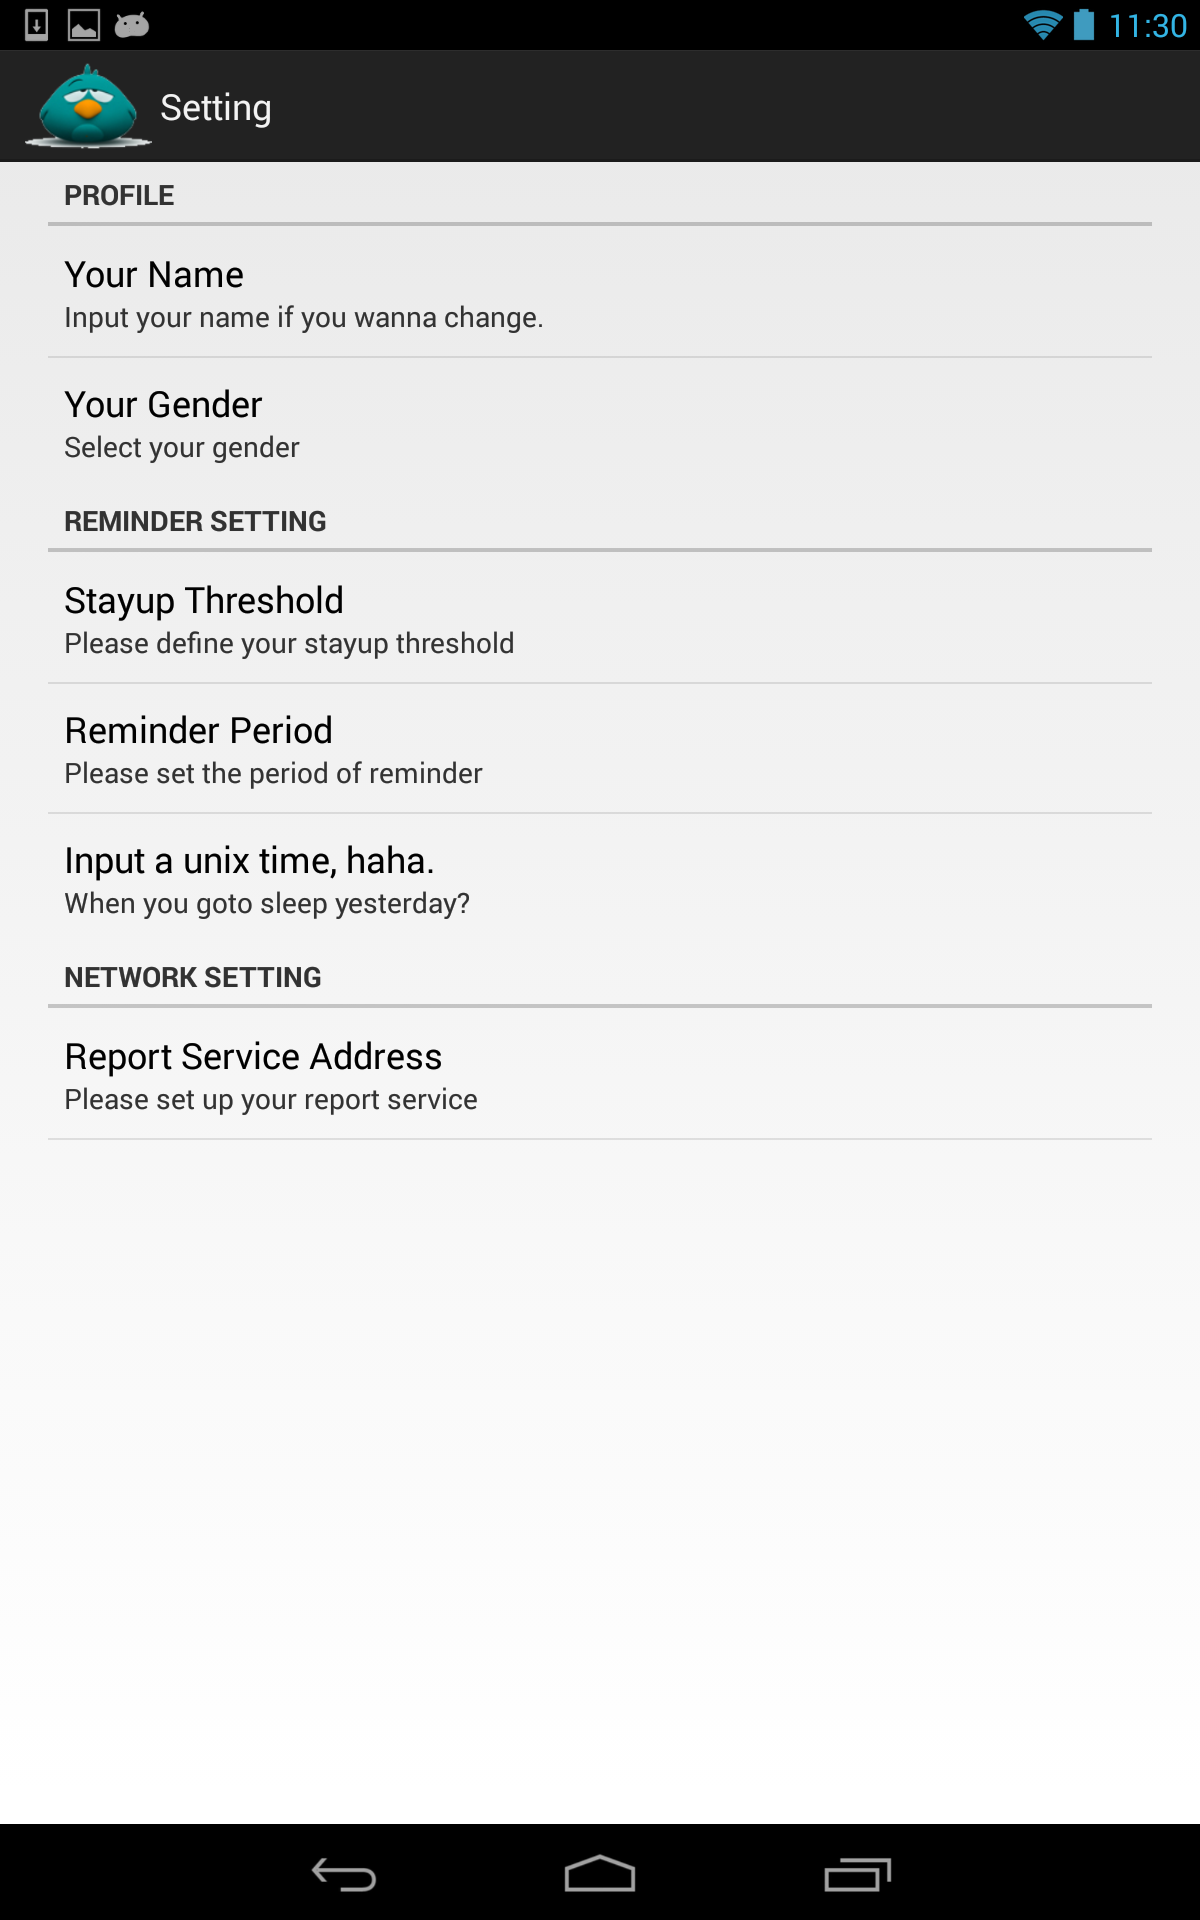
\includegraphics[width=5in]{setting}
\end{center}
\end{figure}

Our provided user preferences are: user's name, gender, user's stay-up-late threshold, period for reminder and server ip for report service as well.

We have a singleton PreferenceManager which provides interfaces to other activities to read and update user's preference programatically. The PreferenceManager invokes android.content.SharedPreferences to read and edit users' settings.

\begin{figure}[h]
\begin{center}
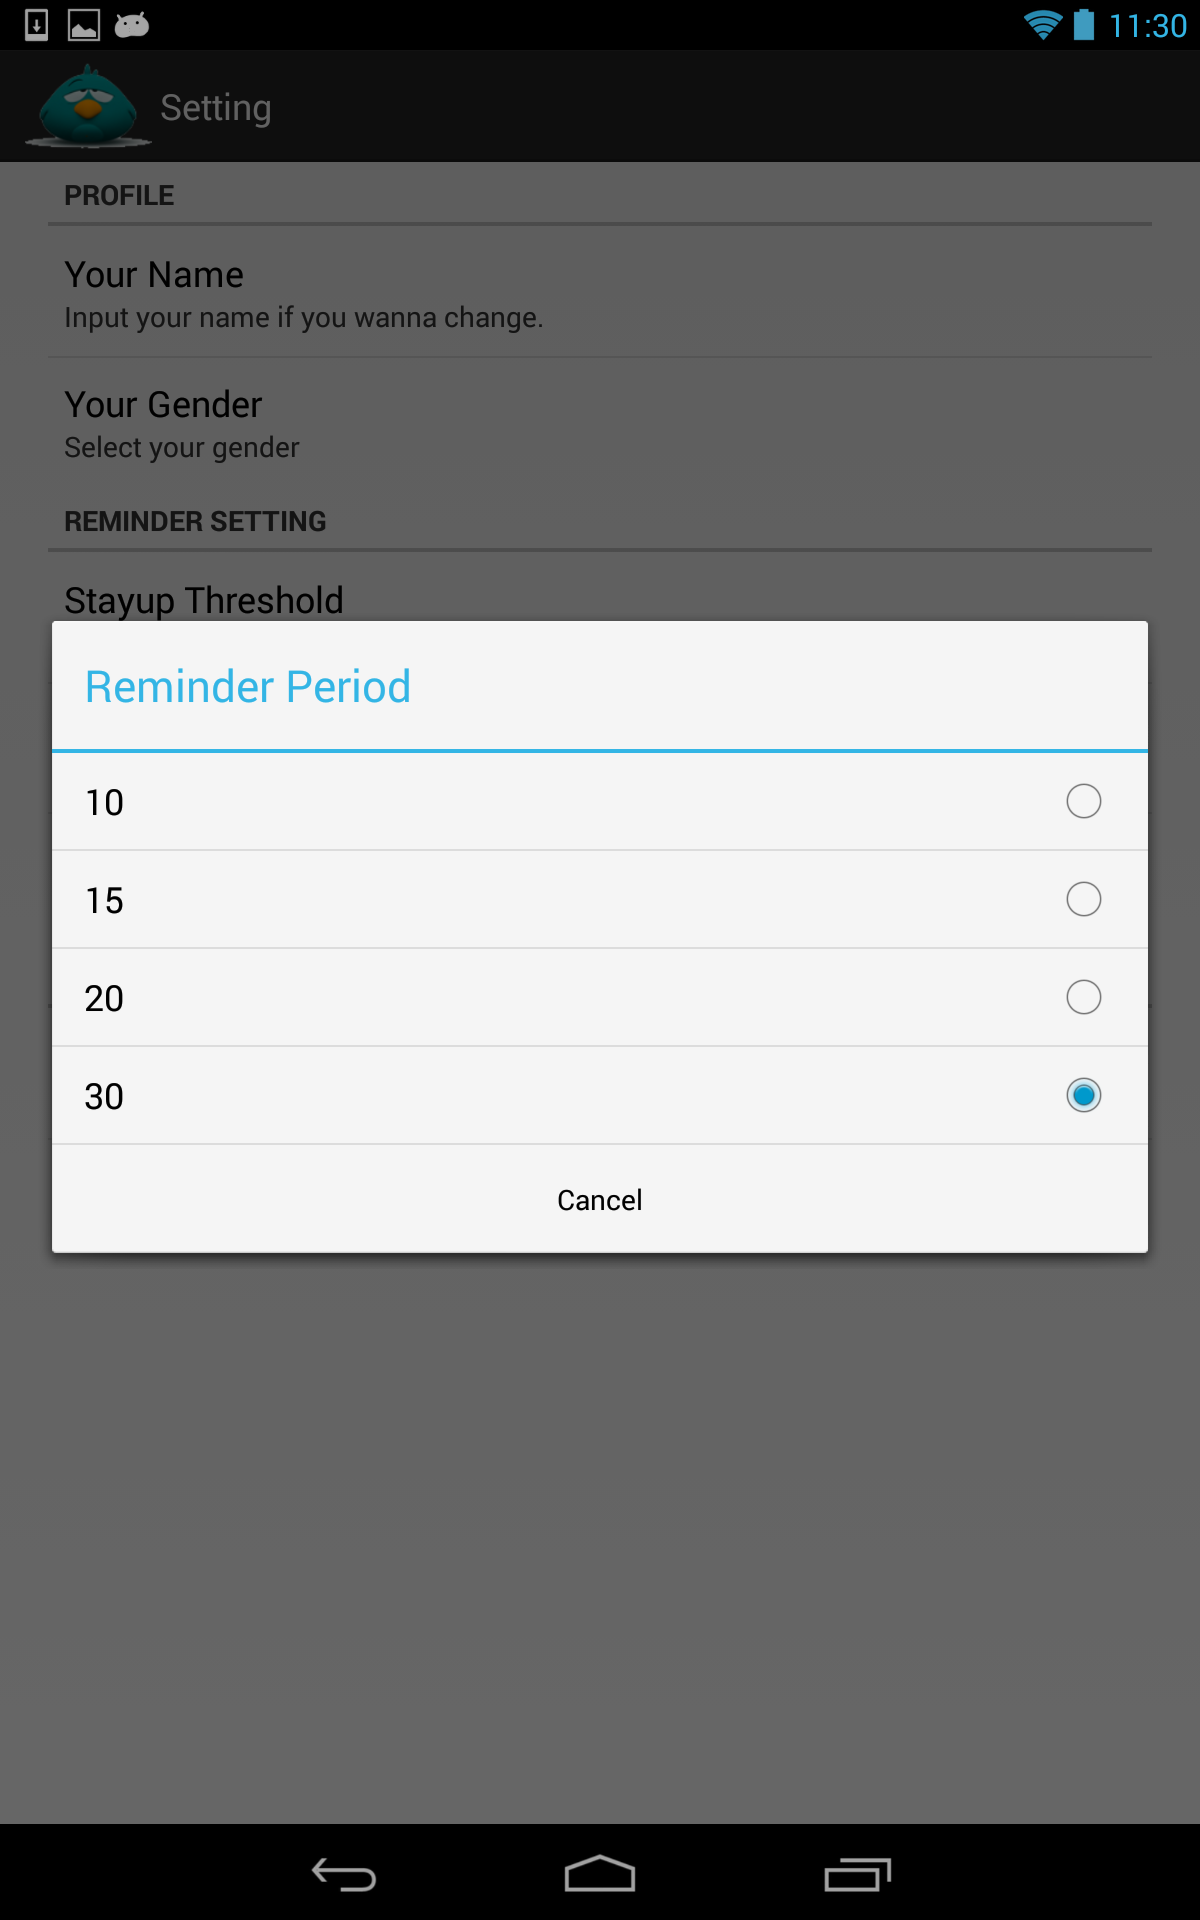
\includegraphics[width=5in]{preference_reminder_period}
\end{center}
\end{figure}


\begin{figure}[h]
\begin{center}
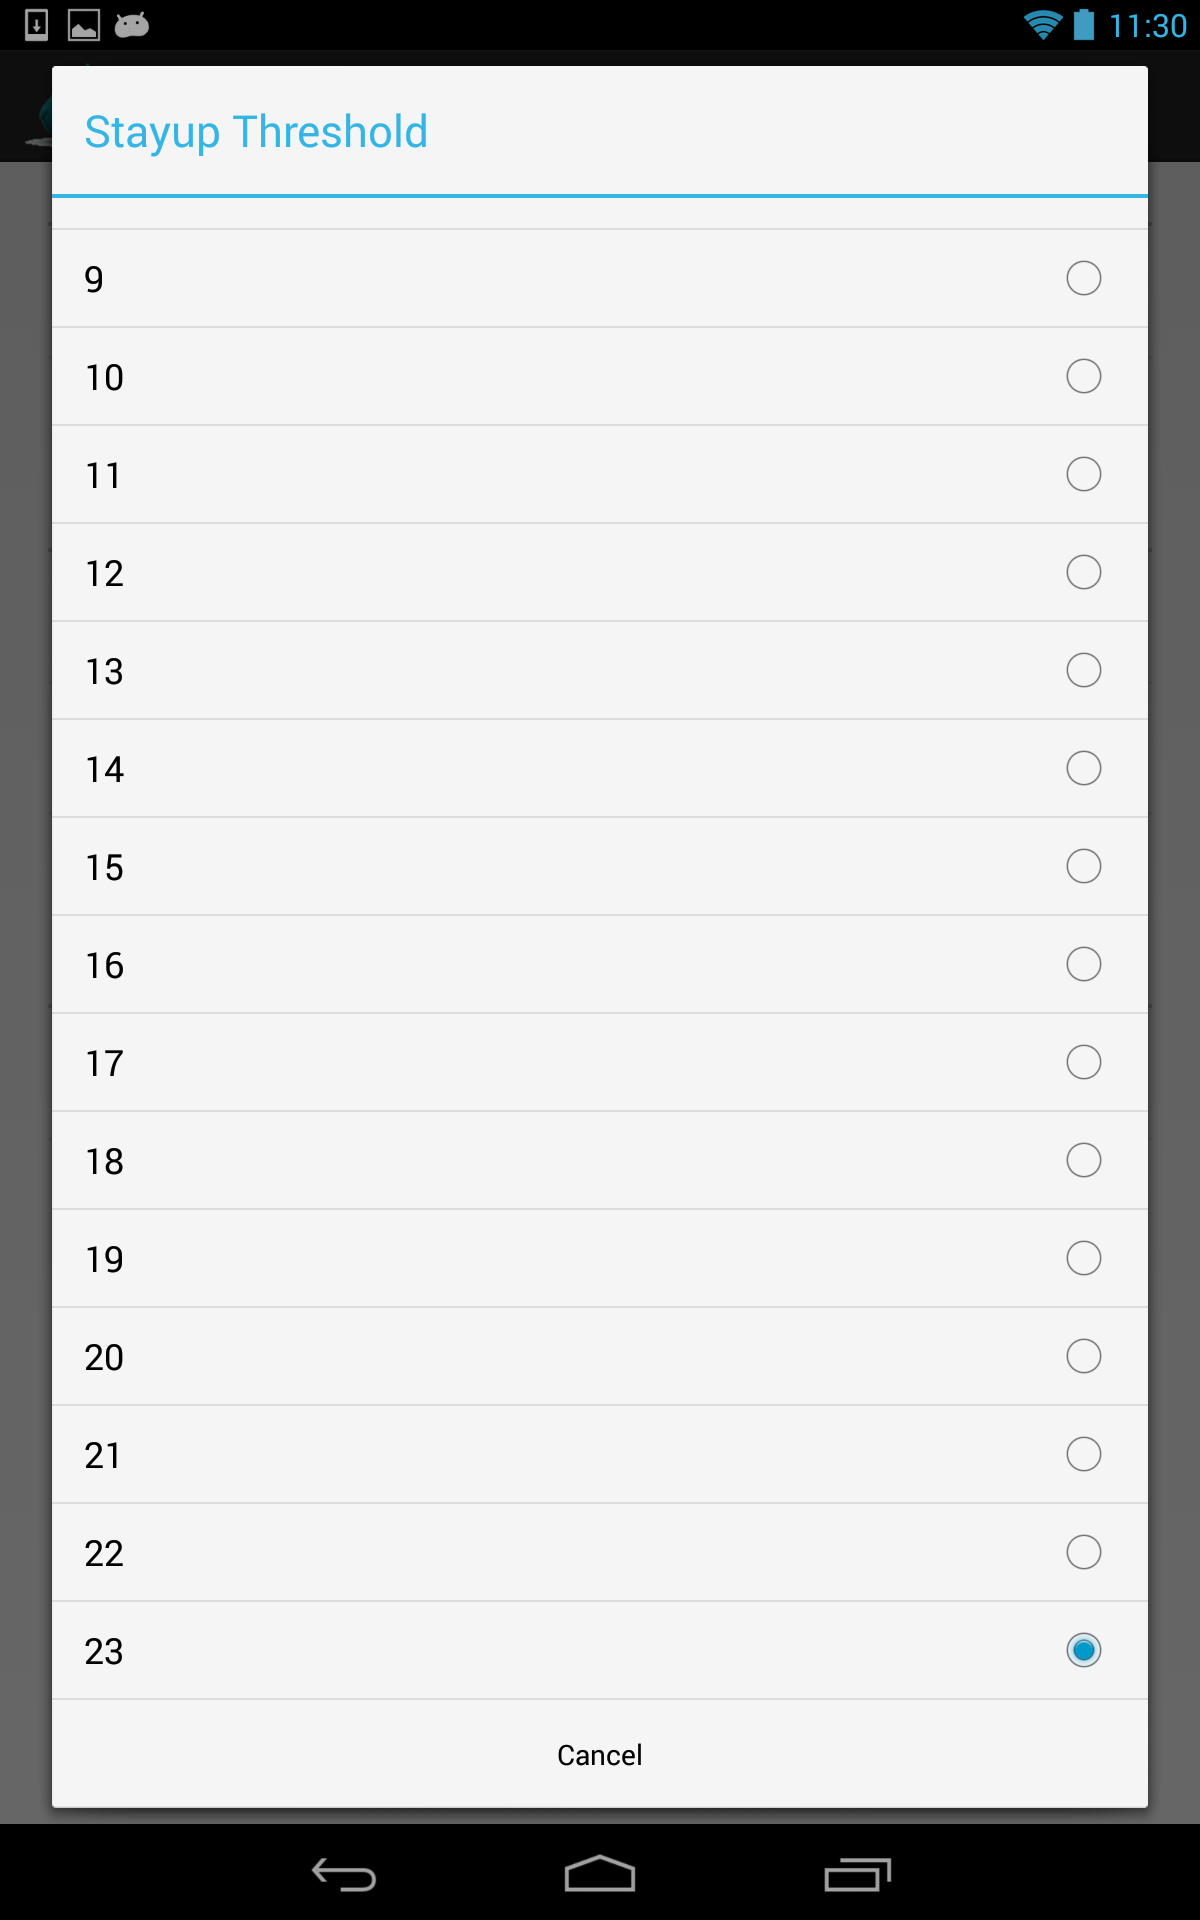
\includegraphics[width=5in]{preference_stayuplate_threshold}
\end{center}
\end{figure}

\chapter{Other Features}
\section{Multiple Resolution Support}
Our application support screens of different resolutions. We use a plugin to generate images for different resolutions. 

\section{Start View}
Start View is controlled in SplashActivity. When the app runs, SplashActivity is created and started. It creates an intent to switch to main activities in few seconds. Before switching to other activity, SplashActivity do initiating works including reading preference from PreferenceManager, configuring StayupReminder and TimeManager, inserting simulation data (used only for debug and demo). 
\begin{figure}[h]
\begin{center}
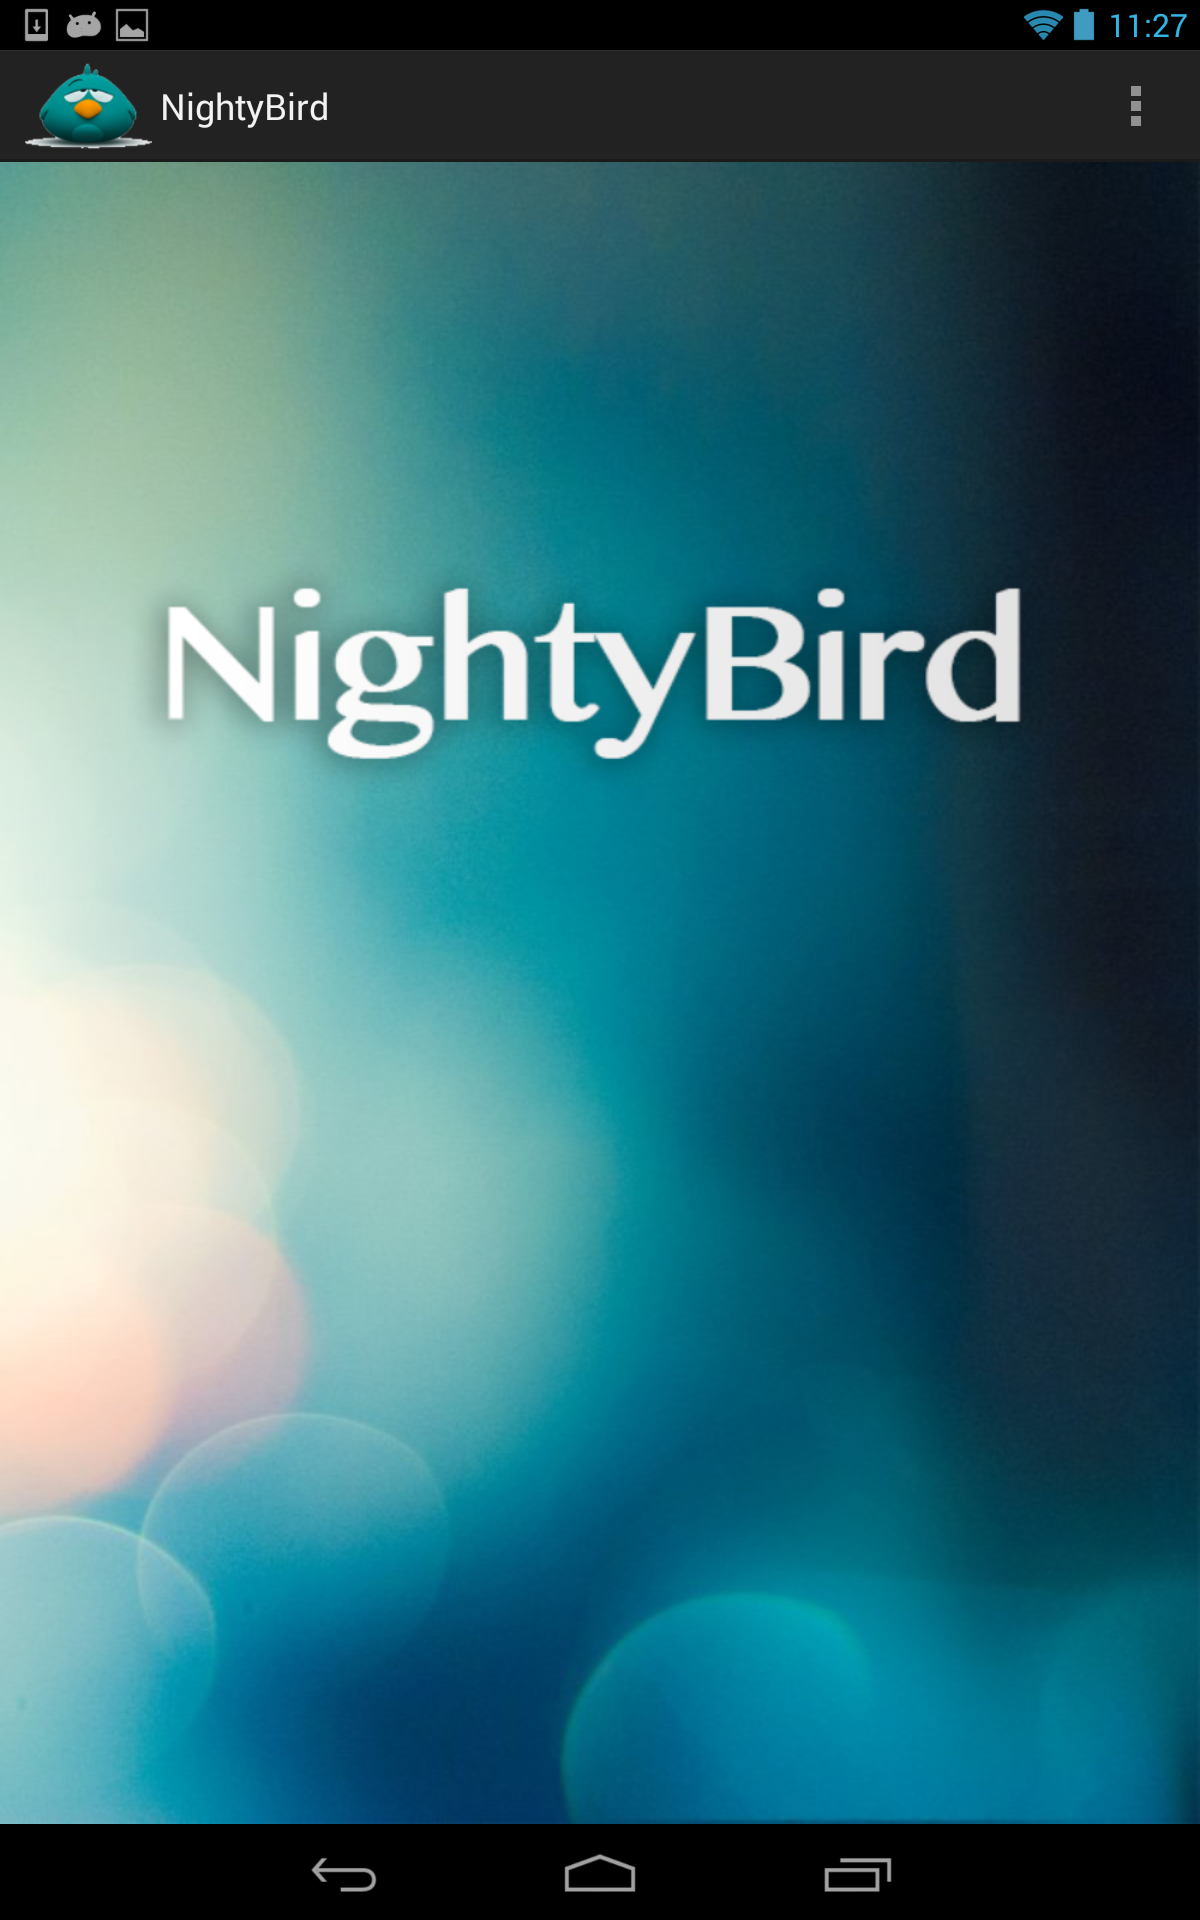
\includegraphics[width=5in]{starview}
\end{center}
\end{figure}

\section{Debugger}
We have a debugger class that makes toast anywhere we want. We use this to debug our application.


\end{document}